\documentclass[a4paper,12pt,reqno]{article}

\usepackage{styledoc19}


\begin{document} % конец преамбулы, начало документа
	
	
	\year{2021}
    \docNumber{RU.17701729.09.09-62 51 01-1}
	\docFormat{Программа и методика испытаний}
	\student{БПИ 174}{Д. Ю. Редникина}
	
	\project{CRM-СИСТЕМА ДЛЯ БЛАГОТВОРИТЕЛЬНОГО ФОНДА <<AIAIN>>. WEB-ПРИЛОЖЕНИЕ ДЛЯ СОТРУДНИКОВ ФОНДА}
	

	\supervisor{Доцент департамента \vfill образовательной программы  \vfill <<Программная инженерия>>}
	{Х. М. Салех}
	
	\firstPage
						\newpage
	\secondPage
						\newpage
	\thirdPage
						\newpage
						
						
	\section{Объекты испытаний}
	\subsection{Наименование программы}
	CRM-система для благотворительного фонда <<AIAIN>>. Web-приложение для сотрудников фонда (System for managing tasks of collecting data from the Internet
)
	\subsection{Область применения программы}
	\subsubsection{Функциональное назначение}
	Система будет применяться как средство управления проектами по созданию, редактированию и запуску веб краулеров для сбора данных в сети интернет. Продукт позволит следить за запусками в режиме реального времени, а также создавать периодические запуски по расписанию.

	\subsubsection{Эксплуатационное назначение}
	Web-приложение является компонентом CRM-системы для благотворительного фонда <<AIAIN>>, позволяющей облегчить бизнес процессы работы фонда с благополучателями и донорами. Web-приложение призвано обеспечить необходимую сотрудникам фонда функциональность для работы с системой. Им будут пользоваться как менеджеры фонда, так и администраторы, члены комиссий, операторы фонда, контент-менеджеры фонда. Каждый из пользователей будет иметь доступ к необходимой ему функциональности по обработке заявок, управлению фондом, администрированию и т.д.
	\subsubsection{Область применения}
	Ежегодно сотни тысяч людей жертвуют свои деньги некоммерческим организациям. Еще больше людей обращаются за помощью в общественные благотворительные фонды. Управлять благотворительным фондом становится все сложнее. Нужно не только принимать пожертвования и регистрировать заявки на сборы средств, но и контролировать работников фонда, волонтеров, подготавливать документацию для вышестоящих органов и многое другое. 

Следовательно, некоммерческие организации нуждаются в платформе с функционалом, ориентированным на бизнес процессы фонда, чтобы обрабатывать всю необходимую информацию в одном месте. К сожалению, большинство фондов пользуются электронными таблицами или, что еще хуже, ведут записи в бумажной форме. Как результат, на каждое действие тратятся большое количество времени и ресурсов. Арабский фонд <<AIAIN>> также столкнулся с проблемой автоматизации бизнес процессов, специфичных для предметной области благотворительности. 


Разрабатываемое Web-приложение ориентировано на специфические нужды некоммерческой организации <<AIAIN>>. Web-приложение для сотрудников фонда может предоставить все преимущества, которыми бизнес-компании пользовались в течение многих лет и чего так не хватало этому фонду. Это также позволит наладить бизнес-процессы внутри фонда <<AIAIN>>, настроить тайм-менеджмент и автоматизировать составление отчетности.
					\newpage
					
	\section{Цель испытаний}
	Проверка на соответствие требованиям, указанным в документе <<CRM-система для благотворительного фонда <<AIAIN>>. Web-приложение для сотрудников фонда. Техническое задание>>.
	
	\section{Требования к программе}
	\subsection{Требования к функциональным характеристикам}
	Программа выполняется в рамках темы выпускной курсовой работы в соответствии с учебным планом подготовки бакалавров по направлению 09.03.04 «Программная инженерия» Национального исследовательского университета «Высшая школа экономики», факультет компьютерных наук.
	
	Программа должна удовлетворять следующим требованиям:
	
	\newlist{subreg}{enumerate}{10}
 
\setlist[subreg, 1]{label=\textbf{FR-\arabic*.}}
\setlist[subreg, 2]{label*=\textbf{\arabic*.}}
\setlist[subreg, 3]{label=\arabic*.}

\begin{subreg}
    \item \label{FR-1} \textbf{Аутентификация\\} 
	Сотрудник фонда должен иметь возможность авторизоваться в системе с логином/паролем, предварительно полученным после регистрации по почте. Процесс регистрации и получения логина/пароля описан в пункте \ref{enum:reg}. Если пользователь не зарегистрирован в системе или авторизуется с неверными данными, то система должна отобразить соответствующее сообщение. 
	
	При первоначальном авторизации в системе на новом устройстве пользователь должен увидеть диалоговое окно с возможностью принять или отклонить получение пуш-уведомлений (подробнее о пуш-уведомлениях в разделе \ref{push}).
	
	\item \textbf{Настройки\\}
    У пользователя должна быть возможность управлять личными данными в настройках системы.
    \begin{subreg} \label{settings}
        \item Должна быть возможность просмотра информации о своем профиле в настройках системы:
        \begin{subreg}
        \item ФИО, почта;
        \item Дата рождения;
        \item Город, страна, телефон;
        \item Фотография;
        \item Роль в системе (см. Приложение \ref{stuff});
        \item Назначенные категории (только для пользователей с ролью <<Член комиссии>>);
        \end{subreg}
        \item Должна быть возможность изменения основной информации:
    \begin{subreg}
        \item ФИО;
        \item Город, страна, телефон;
        \item Фотография;
        \item Дата рождения;
    \end{subreg}
        \item Должна быть возможность выбрать язык системы: русский или английский;
        \item \label{enum:push} Должна быть возможность включить/отключить получение пуш-уведомлений; 
    \end{subreg}
    \item \textbf{Пуш-уведомления\\} \label{push}
    Сотрудники фонда должны иметь возможность получать пуш-уведомления, если такая настройка включена (см. пункт \ref{enum:push}).
    
    \begin{subreg}
        \item Должна быть возможность получения пуш-уведомлений на входящие сообщения в чатах поддержки (для пользователя с ролью <<Оператор>>, подробнее о чатах в пункте \ref{req:chats});
        
        \item Должна быть возможность получения пуш-уведомлений при изменений статусов заявок, которые назначены на конкретного менеджера (для роли <<Менеджер>> и <<Член комиссии>>, подробнее в пункте \ref{req:status});
        
        \item Должна быть возможность получения пуш-уведомлений при изменении статуса операции в системе блокчейн (подробнее в пункте \ref{req:blockchain});
        
        \item Должна быть возможность просмотра списка уведомлений и информации о них:
        \begin{subreg}
        \item Дата и время уведомления;
        \item Тип уведомления;
        \item Инициатор уведомления;
        \end{subreg}
    \end{subreg}
    
    \item \textbf{Статусы операций в системе блокчейн\\} \label{req:blockchain}
    Сотрудники фонда должны иметь возможность просматривать изменения статусов операций в системе блокчейн, а именно: дата, время совершенной операции, тип операции, статус операций, дату, время обновления статуса.
    
    \item \textbf{Управление пользователями\\}
        Этот функционал должен быть доступен только для пользователя с ролью <<Администратор>> (кроме пункта \ref{enum:managers}).
        \begin{subreg}
        \label{admin}
        \item \label{enum:admin_1} Должна быть возможность просмотра информации о пользователе: его ФИО, роль в системе, город, страна, фотография, статус в системе (заблокирован или нет), назначенные категории (только для пользователей с ролью <<Член комиссии>>);
        \item Должна быть возможность изменить все поля из пункта \ref{enum:admin_1}, кроме почты;
        
        \item \label{enum:reg} Должна быть возможность зарегистрировать пользователя в системе, указав:
        \begin{subreg}
            \item ФИО;
            \item Почту;
            \item Роль пользователя в системе (см. Приложение \ref{stuff});
            \item Назначенные категории (только для пользователей с выбранной ролью <<Член комиссии>>);
        \end{subreg}
        После совершения процесса регистрации на указанную почту пользователю приходит логин/пароль для дальнейшей аутентификации в системе;
        \item \label{enum:managers} Должна быть возможность просмотра информации о сотрудниках фонда для пользователя с ролью <<Член комиссии>>: ФИО, роль, город, страна, день рождения, телефон, назначенные категории (если есть), заявки назначенные на пользователя (если есит);
        \end{subreg}
        
    \item \textbf{Логи системы\\}
    У пользователя с ролью <<Администратор>> должна быть возможность просматривать логи системы в формате JSON с обязательными полями: дата регистрации события, тип события и также описание события.
    
    \item \textbf{Транзакции\\}
    Этот функционал должен быть доступен только для пользователя с ролью <<Член комиссии>>.
    \begin{subreg}
        \item Должна быть возможность просматривать транзакции, совершенные внутри системы, информацию о них:
    \begin{subreg}
        \item Дата, время совершения транзакции;
        \item Кто совершил транзакцию (ФИО донора);
        \item Сумма транзакции;
        \item На какую заявку транзакция была совершена - основная информация о заявке: название, автор, тип заявки;
    \end{subreg}
        \item Должна быть возможность провести ручную транзакцию -- вести данные о платеже, поступившем напрямую в фонд. При вводе транзакции должна быть возможность указать цель платежа: на одну из заявок фонда или на нужды фонда, а также ФИО пользователя от которого поступило пожертвование, сумму пожертвования;
    \end{subreg}
    
    \item \textbf{Категории\\}
    Этот функционал должен быть доступен только для пользователя с ролью <<Член комиссии>>.
    \begin{subreg}
        \item Должна быть возможность просматривать категории фонда, доступные для назначения на заявки, а именно:
        \begin{subreg}
            \item ID - уникальный идентификатор категории;
            \item Название категории на английском;
            \item Название категории на русском языке;
            \item Название категории на арабском;
            \item Видимость категории - некоторые категории должны быть скрыты от пользователей при назначении категории на заявку;
        \end{subreg}
        \item Должна быть возможность изменить все данные о категориях;
        \item Должна быть возможность удалить категорию. Для удаления доступны только те категории, которые не используются в системе (т.е не назначены на пользователей или на заявку);
    \end{subreg}
    
    \item \textbf{Заявки\\}
    Эта функциональность должна быть доступна для пользователей с ролью <<Член комисии>> и <<Менеджер>>;
    \begin{subreg}
    \item \label{req:status} Должна быть возможность изменять статусы заявок в зависимости от роли пользователя и предыдущего статуса заявки в соответствии с диаграммой жизненного цикла заявки (см. Приложение \ref{status});
    \item Должна быть возможность отредактировать данные о заявке (одобренная сумма, срок сбора средств), когда она находится в статусе <<В обработке>>; 
    \item Должна быть возможность создать заявку в системе от лица незарегистрированного пользователя. При создании заявки нужно указать: название,  описание, сумма сбора, категория заявки, документы и дата сбора. Заявка сразу создается в статусе <<Активная>> от имени фонда. Эта функциональность должна быть доступна только для пользователей с ролью <<Член комиссии>>;
    \item Должна быть возможность оставлять комментирии к заявке;
    \item Должна быть возможность просматривать комментарии к заявке: текст сообщения, дату и автора;
    \item Должна быть возможность менять менеджера, который назначен на обработку заявки;
    \item Должна быть возможность закрыть сбор средств на заявку;
    \item Должна быть возможность просмотреть информацию о голосовании по заявке в статусе <<Ждет подтверждения члена комиссии>>, а именно: кто имеет право проголосовать и их решение, а также статус голосования (в процессе, принято, отклонено);
    \item У пользователей с ролью <<Член комиссии>> должна быть возможность проголосовать по заявке (за принятие или против), если категория заявки совпадает с назначенной на члена комиссии категорией;
    \end{subreg}
    
    \item \textbf{Чаты\\} \label{req:chats}
    Данная функциональность должна быть доступна только пользователям с ролью <<Оператор>>;

    \begin{subreg}
    \item Должна быть возможность просматривать список чатов: ФИО собеседника, текст сообщения, количество непрочитанных сообщений;
    \item Должна быть возможность написать сообщение;
    \end{subreg}
    
    \item \textbf{Управление контентом фонда\\}
    Данная функциональность должна быть доступна только для пользователей с ролью <<Контент-менеджер>>;
    
    \begin{subreg}
    \item Должна быть возможность просмотривать м редактировать часто задаваемые вопросы в формате \texttt{markdown} \cite{md};
    \item Должна быть возможность просмотривать, редактировать, удалять и создавать новости фонда. Для создания нужно указать название, описание новости и фотографию;
    \item Должна быть возможность просмотра и редактирования информации о фонде: описания и загруженных документов;
    \end{subreg}
    
\end{subreg}


\renewcommand{\labelenumi}{\arabic{enumi}.}

\renewcommand{\labelenumii}{\arabic{enumii}.}

\renewcommand{\labelenumiii}{\arabic{enumiii}.}





	
	\subsection{Требования к интерфейсу}
	Цветовая гамма интерфейса должена быть выполнена в голубых тонах. Разработанный интерфейс должен соответствовать макетам (см. Приложение \ref{figma}).
	
	\subsection{Требования к надежности}
	
	\newlist{nfr}{enumerate}{10}
 
    \setlist[nfr, 1]{label=\textbf{NFR-\arabic*.}}
    \setlist[nfr, 2]{label*=\textbf{\arabic*.}}
    \setlist[nfr, 3]{label=\arabic*.}
	
	\begin{nfr}
	    \item Система должна сохранять работоспособность и обеспечивать восстановление своих функций при возникновении следующих внештатных ситуаций:
	    \begin{nfr}
	    \item При ошибках работы сервера, к которому по API отправляет запросы Web-приложение, программа должна отображать сообщения в формате уведомлений в UI и продолжать корректную работу;
        \item При ошибках в сбоях аппаратных средств (кроме носителей данных) восстановление работоспособности возлагается на ОС;
        \item При ошибках, связанных с веб-браузером, восстановление работоспособности возлагается на ОС;
	\end{nfr}
	\item Компоненты защиты программы от несанкционированного доступа к данным и функционалу должны обеспечивать:
	\begin{nfr}
	\item Идентификацию пользователя;
	\item Проверку полномочий пользователя при работе с системой;
	\item Разграничение прав доступа пользователей на уровне задач и доступа к данным;
    \end{nfr}
	\end{nfr}
    
    \section{Требования к программной документации}
	\subsection{Состав программной документации}
	Состав программной документации должен включать в себя следующие компоненты:
\begin{enumerate}
	\item Техническое задание <<CRM-система для благотворительного фонда <<AIAIN>>. Web-приложение для сотрудников фонда>> (ГОСТ 19.201-78) \label{tz}
	\item Программа и методика испытаний <<CRM-система для благотворительного фонда <<AIAIN>>. Web-приложение для сотрудников фонда>> (ГОСТ 19.301-78) \label{pmi}
	\item Руководство оператора <<CRM-система для благотворительного фонда <<AIAIN>>. Web-приложение для сотрудников фонда>> (ГОСТ 19.505-79) \label{ro}
	\item Текст программы <<CRM-система для благотворительного фонда <<AIAIN>>. Web-приложение для сотрудников фонда>> (ГОСТ 19.401-78) \label{tp}
\end{enumerate}

\indent
Вся документация должна быть составлена согласно ЕСПД (ГОСТ 19.101-77, 19.104-78, 19.105-78, 19.106-78 и ГОСТ к соответствующим документам (см. выше)) \cite{gost}. Все документы сдаются в электронном виде в составе выпускной квалификационной работы LMS НИУ ВШЭ.

% Пояснительная записка <<CRM-система для благотворительного фонда <<AIAIN>>. Web-приложение для сотрудников фонда>> должна быть проверена на плагиат ($< 40\% $ заимствований). Документ, подтвержадющий проверку Пояснительной записки сдается в печатном виде вместе с подписанным отзывом от научного руководителя.

	
	\newpage
	\section{Средства и порядок испытаний}
	\subsection{Технические средства, используемые во время испытаний}
	\begin{enumerate}
        \item Компьютер оснащенный процессором Intel Core i5 с тактовой частотой 2,3 ГГц;
        \item 16 Гб ОЗУ;
        \item Жесткий диск с объемом свободной памяти более чем 50 ГБ;
        \item Клавиатура и мышь;
        \item Доступ в интернет.
\end{enumerate}
	\subsection{Программные средства, используемые во время испытаний}
	\begin{enumerate}
        \item macOS 10.15.2;
        \item scrapyd~\cite{scrapyd};
        \item Scala 2.12.6;
        \item Play-framework 2.6.13;
        \item PostgreSQL 11~\cite{postgresql};
    \end{enumerate}
	Тестирование производилось с развернутым Web-приложением и API~\cite{api} на стенде, по адресу \url{https://charity.infostrategic.com/}.
	
	
	\subsection{Порядок проведения испытаний}
	В процессе разработки программы были написаны unit-тесты, а также автотесты, тестирующие интеграционное взаимодействие Web-клиента и сервера~\cite{api}.
	
	Unit-тесты были написаны с помощью фреймворка Jest~\cite{jest}. При разработке приложения был использован сервис Gitlab, а также встроенный в Gitlab механизм CI/CD~\cite{cicd}. Разработка была построена следующим образом: на каждом коммите в пулл реквесте запускался пайплайн, который состоял из следующих этапов: Eslint, Prettier, Test. Первые два шага - линтеры, которые осуществляли проверку файлов проекта на код-стайл. На последнем этапе пайплана запускались unit-тесты проекта.
	
	Для автоматизации тестирования UI использовался фреймворк Silenium IDE~\cite{silenium}. С помощью этого фреймворка были написаны интеграционные авто-тесты, покрывающие основные бизнес-требования, отраженные на диаграмме прецедентов в Приложении. \ref{keyUsecase}.
	
	\newpage
	\section{Методы испытаний}
	
	Этап Test пайаплайна CI/CD автоматически запускает тесты проекта с помощью команды: \texttt{yarn test}. На изображении \ref{pic: test} можно увидеть успешный результат прохождения тестов в проекте.
	
	\begin{figure}[H]
		\centering
		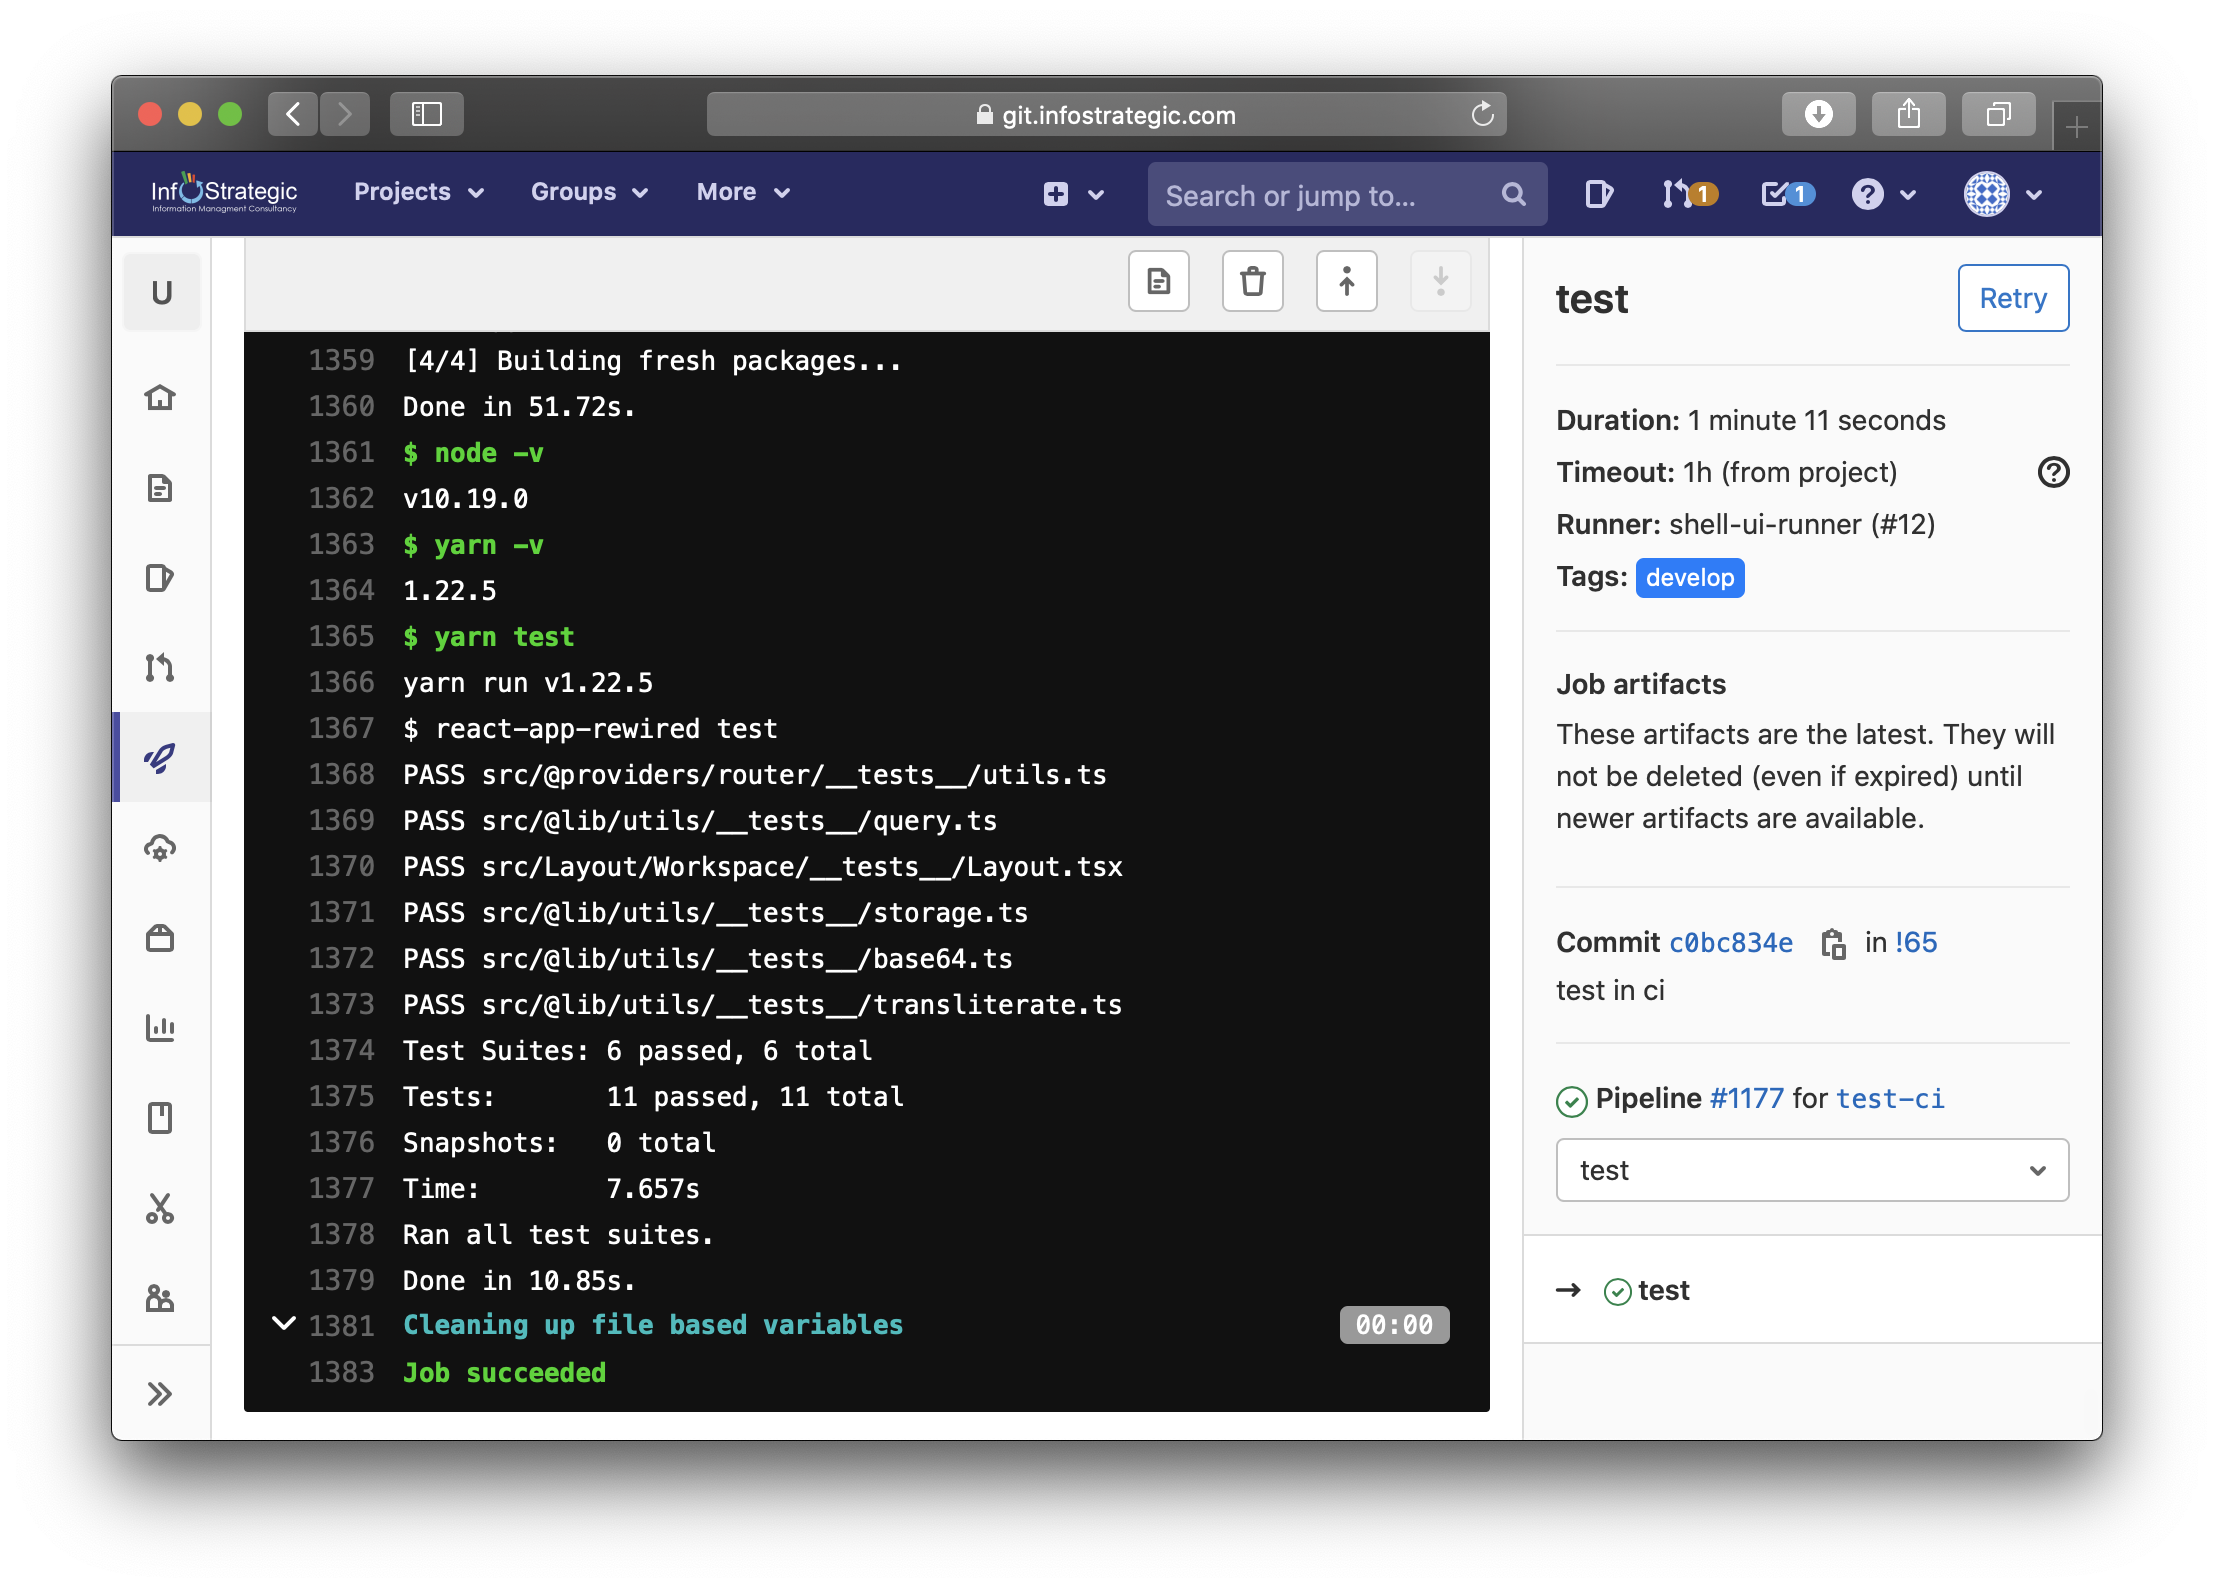
\includegraphics[width = \linewidth]{img/test.png}
		\caption{Тестирование. CI job.}
		\label{pic: test}
	\end{figure}
	
	
	\subsection{Проверка требований к функциональным характеристикам}
	
	При тестировании Веб-приложения был использован фреймворк Silenium IDE~\cite{silenium}. С помощью плагина, установленного в браузер Google Chrome~\cite{chrome}, были записаны тесты, проверяющие удовлетворение проекта составленным требованиям.
	
	Для тестирования ключевых бизнес-процессов, выделенных на диаграмме прецедентов цветом (см. Приложение \ref{keyUsecase}), были составлены следующие тест-кейсы. По данным тест-кейсам были созданы тесты Silenium:
	
	\renewcommand{\labelenumi}{\textbf{TC-\arabic{enumi}}.}

\renewcommand{\labelenumii}{\textbf{TC-\arabic{enumi}.\arabic{enumii}}.}


\begin{enumerate}
    \item Авторизация;
    
    \begin{enumerate}
        \item Авторизация зарегистрированного пользователя в системе;
        
        \textbf{Предусловие}: Пользователь зарегистрирован в системе и имеет роль <<Оператор>>, <<Менеджер>>, <<Член комиссии>>, <<Администратор>> или <<Контент-менеджер>>, но не авторизован в системе; 
    
        \textbf{Постусловие}: Пользователь успешно авторизован в системе и имеет доступ к функционалу, соответствующего его роли;
        
        \textbf{Описание}: Пользователь открывает страницу веб-приложения с URL: \url{https://charity.infostrategic.com/login} и вводит логин/пароль, с которым был ранее зарегистрирован;
        
        \textbf{Ожидаемый результат}: Пользователь попадает на страницу с URL: \url{https://charity.infostrategic.com/applications} (если пользователь имеет роль <<Менеджер>>,  <<Член комиссии>>), URL: \url{https://charity.infostrategic.com/chats} (если пользователь имеет роль <<Оператор>>), URL: \url{https://charity.infostrategic.com/fund/description} (если пользователь имеет роль <<Контент-менеджер>>), URL: \url{https://charity.infostrategic.com/users} (если пользователь имеет роль <<Администратор>>); В хэдерах приложения должен быть токен \texttt{Authorization}.
        
        \textbf{Требования, покрываемые тест кейсом}: FR-1;
        
        \textbf{Покрытые юзкейсы}: Sign In;
        
        \item Авторизация незарегистрированного пользователя в системе;
        
        \textbf{Предусловие}: Пользователь не зарегистрирован в системе; 
    
        \textbf{Постусловие}: Пользователь не авторизован в системе;
        
        \textbf{Описание}: Пользователь открывает страницу веб-приложения с URL: \url{https://charity.infostrategic.com/login} и вводит любой логин/пароль;
        
        \textbf{Ожидаемый результат}: Система отображает уведомление с текстом <<Вы не зарегистированы в системе>>;
        
        \textbf{Покрытые требования}: FR-1;
        
        \textbf{Покрытые юзкейсы}: Sign In;
    \end{enumerate}
    
    \item Настройки;
    \begin{enumerate}
        \item Изменение настроек профиля пользователя;
        
        \textbf{Предусловие}: Пользователь авторизован в системе;
        
        \textbf{Постусловие}: Пользователь изменил информацию о своем профиле;
        
        \textbf{Описание}: Авторизованный пользователь переходит на URL: \url{https://charity.infostrategic.com/settings} и меняет: фотографию, ФИО, телефон, адрес, город, страну. После изменения информации пользователь нажимает кнопку <<Сохранить изменения>>.
        
        \textbf{Ожидаемый результат}: Система отображает оповещение <<Все изменения успешно сохранены>>, пользователь видит новые данные в том же разделе.
        
        \textbf{Покрытые требования}: FR-2 (FR-2.1, FR-2.2);
        
        \textbf{Покрытые юзкейсы}: Update and read profile;
        
        \item Изменение языка системы;
        
        \textbf{Предусловие}: Пользователь авторизован в системе;
        
        \textbf{Постусловие}: Пользователь изменил язык системы;
        
        \textbf{Описание}: Авторизованный пользователь переходит на URL: \url{https://charity.infostrategic.com/settings} и меняет язык системы.
        
        \textbf{Ожидаемый результат}: Система отображает оповещение <<Язык системы успешно изменен>>, система меняет надписи на соответствующие выбранному языку.
        
        \textbf{Покрытые требования}: FR-2 (FR-2.3);
        
        \textbf{Покрытые юзкейсы}: Update and read profile;
    \end{enumerate}
    
    \item Управление пользователями;
    \begin{enumerate}
        \item Регистрация пользователя в системе;
        
        \textbf{Предусловие}: Пользователь авторизован в системе под аккаунтом с ролью <<Администратор>>;
        
        \textbf{Постусловие}: Новый пользователь зарегистрирован в системе;
        
        \textbf{Описание}: Авторизованный пользователь переходит на URL: \url{https://charity.infostrategic.com/users/create} и заполняет ФИО будущего пользователя, а также указывает его email и роль в системе.
        
        \textbf{Ожидаемый результат}: Система отображает оповещение <<Пользователь успешно зарегистрирован>> и перебрасывает на URL:\\ \url{https://charity.infostrategic.com/users}, где можно увидеть данные о только что зарегистрированном пользователе.
        
        \textbf{Покрытые требования}: FR-4 (FR-4.3);
        
        \textbf{Покрытые юзкейсы}: CRU of users;
    \end{enumerate}
    
    \begin{enumerate}
        \item Просмотр и изменение профиля пользователя;
        
        \textbf{Предусловие}: Пользователь авторизован в системе под аккаунтом с ролью <<Администратор>>;
        
        \textbf{Постусловие}: Данные о пользователе обновлены;
        
        \textbf{Описание}: Авторизованный пользователь переходит на URL: \url{https://charity.infostrategic.com/users/id}, где id - ID одного из пользователей в системе. Администратор меняет поля ФИО, роль, назначенные категории (если есть);
        
        \textbf{Ожидаемый результат}: Система отображает оповещение <<Информация о пользователе успешно изменена>> и перебрасывает на URL: \url{https://charity.infostrategic.com/users}, где можно увидеть измененные данные о пользователе.
        
        \textbf{Покрытые требования}: FR-4 (FR-4.1, FR-4.2);
        
        \textbf{Покрытые юзкейсы}: CRU of users;
    \end{enumerate}
    
    \item Управление новостным контентом;
    
    \begin{enumerate}
        \item Просмотр и изменение новостей фонда;
        
        \textbf{Предусловие}: Пользователь авторизован в системе под аккаунтом с ролью <<Контент-менеджер>>;
        
        \textbf{Постусловие}: Список новостей обновлен;
        
        \textbf{Описание}: Авторизованный пользователь переходит на URL: \url{https://charity.infostrategic.com/news}, где виден список новостей фонда. Далее пользователь переходит на URL: \url{https://charity.infostrategic.com/news/id} где id - ID одной из новостей в системе. Контент-менеджер меняет картинку, название, описание новости и нажимает кнопку <<Сохранить изменения>>;
        
        \textbf{Ожидаемый результат}: Система отображает оповещение <<Информация о новости успешно изменена>> и перебрасывает на URL: \url{https://charity.infostrategic.com/news}, где можно увидеть измененные новости.
        
        \textbf{Покрытые требования}: FR-10 (FR-10.2);
        
        \textbf{Покрытые юзкейсы}: CRUD news;
    \end{enumerate}
    
    \begin{enumerate}
        \item Удаление новости фонда;
        
        \textbf{Предусловие}: Пользователь авторизован в системе под аккаунтом с ролью <<Контент-менеджер>>;
        
        \textbf{Постусловие}: Выбранная новость удалена;
        
        \textbf{Описание}: Авторизованный пользователь переходит на URL: \url{https://charity.infostrategic.com/news}, где виден список новостей фонда. Из списка новостей пользователь удаляет выбранную.
        
        \textbf{Ожидаемый результат}: Система отображает оповещение <<Новость успешно удалена>> и можно увидеть, что удаленной новости в списке больше нет.
        
        \textbf{Покрытые требования}: FR-10 (FR-10.2);
        
        \textbf{Покрытые юзкейсы}: CRUD news;
    \end{enumerate}
    
    \item Чат поддержки;
    
    \begin{enumerate}
        \item Просмотр диалогов с пользователями;
        
        \textbf{Предусловие}: Пользователь авторизован в системе под аккаунтом с ролью <<Оператор>>;
        
        \textbf{Постусловие}: -
        
        \textbf{Описание}: Авторизованный пользователь переходит на URL: \url{https://charity.infostrategic.com/chats}. В списке можно увидеть сообщения от пользователей, которые обновляются в режиме реального времени. Можно увидеть следующую информацию о чате: ФИО собеседника, текст последнего сообщения;
        
        \textbf{Ожидаемый результат}: Чаты обновляются в режиме реального времени;
        
        \textbf{Покрытые требования}: FR-9 (FR-9.1);
        
        \textbf{Покрытые юзкейсы}: CRU support chats;
    \end{enumerate}
    
    \begin{enumerate}
        \item Написать сообщение пользователю;
        
        \textbf{Предусловие}: Пользователь авторизован в системе под аккаунтом с ролью <<Оператор>>;
        
        \textbf{Постусловие}: Сообщение пользователю отправлено;
        
        \textbf{Описание}: Авторизованный пользователь переходит на URL: \url{https://charity.infostrategic.com/chats}. В списке чатов пользователь выбирает диалог и нажимает на него. В текстовом поле оператор набирает сообщение и отправляет пользователю, нажав кнопку <<Отправить>>; 
        
        \textbf{Ожидаемый результат}: Отправленное сообщение появляется в диалоге с пользователем;
        
        \textbf{Покрытые требования}: FR-9 (FR-9.2);
        
        \textbf{Покрытые юзкейсы}: CRU support chats;
    \end{enumerate}
    
    \item Регистрация и просмотр пожертвовании;
    
    \begin{enumerate}
        \item Регистрация пожертвования фонду;
        
        \textbf{Предусловие}: Пользователь авторизован в системе под аккаунтом с ролью <<Член комиссии>>;
        
        \textbf{Постусловие}: Пожертовование зарегистрировано в системе;
        
        \textbf{Описание}: Авторизованный пользователь переходит на URL: \url{https://charity.infostrategic.com/transactions/create}. После заполнения необходимых полей формы, пользователь нажимает кнопку <<Создать транзакцию>>. 
        
        \textbf{Ожидаемый результат}: Зарегистрированная транзакция появляется в системе;
        
        \textbf{Покрытые требования}: FR-6 (FR-6.1, FR-6.2);
        
        \textbf{Покрытые юзкейсы}: Create donation, Read donation;
    \end{enumerate}
    
    \item Категории заявок;
    
    \begin{enumerate}
        \item Создание, изменение и просмотр категорий;
        
        \textbf{Предусловие}: Пользователь авторизован в системе под аккаунтом с ролью <<Член комиссии>>;
        
        \textbf{Постусловие}: Категории фонда обновлены;
        
        \textbf{Описание}: Авторизованный пользователь переходит на URL: \url{https://charity.infostrategic.com/categories}. В UI отображается информация об уже зарегистрированных категориях: ID, название на английском, название на русском и арабском языках, а также галочка - скрыта ли категория. Пользователь добавляет категории и всю необходимую информацию. Пользователь нажимает кнопку <<Сохранить изменения>>;
        
        \textbf{Ожидаемый результат}: Появляется уведомление <<Категории успешно обновлены>>;
        
        \textbf{Покрытые требования}: FR-7 (FR-7.1, FR-7.2, FR-7.3);
        
        \textbf{Покрытые юзкейсы}: CRUD categories;
    \end{enumerate}
    
    \item Просмотр сотрудников фонда;
    
    \begin{enumerate}
        \item Просмотр сотрудников фонда;
        
        \textbf{Предусловие}: Пользователь авторизован в системе под аккаунтом с ролью <<Член комиссии>>;
        
        \textbf{Постусловие}: -
        
        \textbf{Описание}: Авторизованный пользователь переходит на URL: \url{https://charity.infostrategic.com/managers}. 
        
        \textbf{Ожидаемый результат}: В UI отображается информация о сотрудниках фонда с ролями <<Менеджер>>, <<Член комиссии>>, <<Контент-менеджер>>, <<Оператор>>: ФИО, почта, роль. Перейдя на одну из страниц менеджера должна быть видна следующая информация: ФИО, фотография профиля, роль пользователя, заявки, назначенные на пользователя;
        
        \textbf{Покрытые требования}: FR-4 (FR-4.4);
        
        \textbf{Покрытые юзкейсы}: View managers;
    \end{enumerate}
\end{enumerate}



\renewcommand{\labelenumi}{\arabic{enumi}.}


\renewcommand{\labelenumii}{\arabic{enumii}.}
	
	Результаты UI тестов Silenium можно увидеть на рисунке \ref{pic: silenium}
	
	\begin{figure}[H]
		\centering
		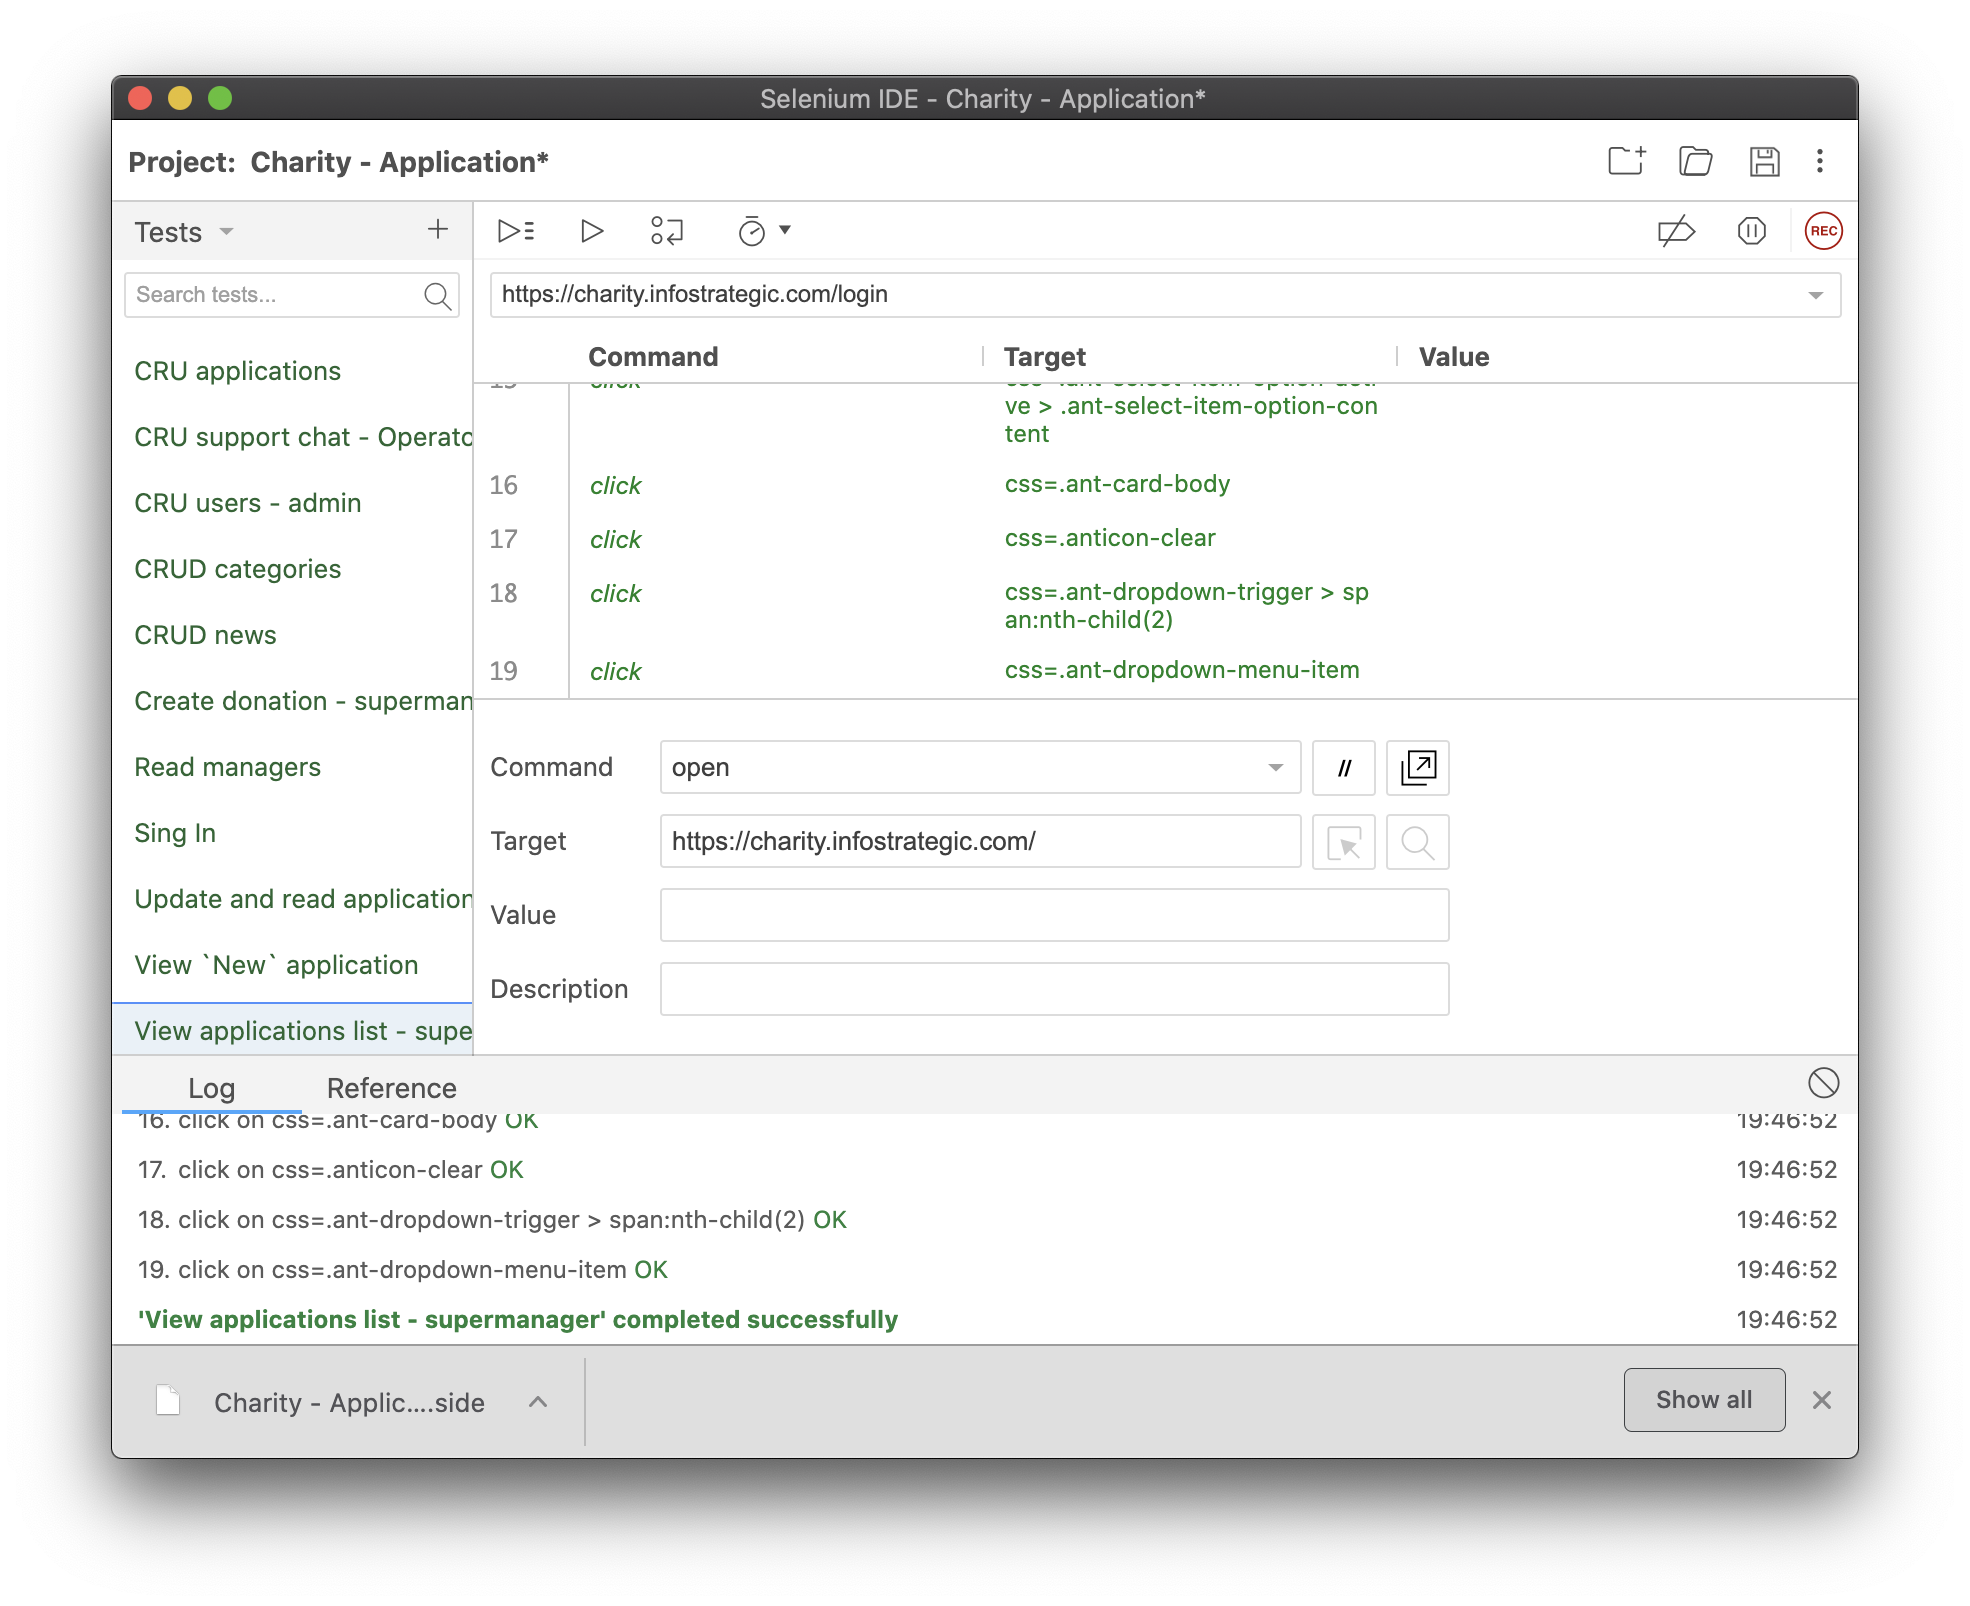
\includegraphics[width = \linewidth]{img/silenium.png}
		\caption{Silenium IDE. Проект с тестами}
		\label{pic: silenium}
	\end{figure}
	
	Также было проведено регрессионное ручное тестирование сложных и многоэтапных бизнес-процессов, включающих активацию заявки и голосование по заявке. Данные сценарии невозможно автоматизировать с помощью Silenium IDE, так как их невозможно завершить (проверить полностью) без использования Android-клиента (или совершения запросов через консоль-клиент). 
	
	Для проверки требований и бизнес-сценариев были написаны следующие тест-кейсы:
	
	\renewcommand{\labelenumi}{\textbf{TC-\arabic{enumi}}.}

\renewcommand{\labelenumii}{\textbf{TC-\arabic{enumi}.\arabic{enumii}}.}


\begin{enumerate}
    \setcounter{enumi}{8}
    \item Обработка заявки;
    
    \begin{enumerate}
        \item Обработка заявки членом комиссии;
        
        \textbf{Предусловие}: Пользователь авторизован в системе под аккаунтом с ролью <<Член комиссии>>; Есть хотя бы одна заявка в статусе <<Новая>>;  
        
        \textbf{Постусловие}: Заявка в статусе <<Активна>>;
        
        \textbf{Описание}: \begin{enumerate}
            \item Член комисии переходит на карточку заявки в статусе <<Новая>>;
            \item Член комисии открывает с помощью кнопки в правом углу <<Действия с заявкой>> панель, в которой должна быть обеспечеа возможность выбора следующего статуса для заявки в соответствии с диаграммой, представленной в Приложении \ref{status}.
            \item Член комисии выбирает статус <<В обработке>> и нажимает кнопку <<Подтвердить>>; 
            \item После закрытия панели статус в карточке заявки должен смениться статус на <<В обработке>> и появиться уведомление об успехе операции;
            \item Член комиссии нажимает кнопку <<Изменить>> и редактирует одобренную сумму для сбора;
            \item Далее нужно повторить шаги 2-4 и выбрать новый статус <<Ждет подтверждения>>;
            \item После того, как все члены комиссии проголосовали за активацию заявки должен быть доступен в панели статус <<Ждет активации пользователя>>;
            \item После активации заявки с мобильного устройства пользователем, создавшим заявку (или через консоль-клиент) статус обрабатываемой заявки становится <<Активна>>;
        \end{enumerate}
        
        \textbf{Ожидаемый результат}: Статус заявки будет <<Активна>>;
        
        \textbf{Покрытые требования}: FR-8 (FR-8.1, FR-8.7);
        
        \textbf{Покрытые юзкейсы}: Approve application;
        
        \item Голосование по заявке;
        
        \textbf{Предусловие}: Пользователь авторизован в системе под аккаунтом с ролью <<Член комиссии>>; Есть хотя бы одна заявка в статусе <<Ждет подтверждения>> с категорией, совпадающей с категорией назначенной на члена комиссии;  
        
        \textbf{Постусловие}: Заявка может быть переведена в статус <<Ждет активации>>;
        
        \textbf{Описание}: \begin{enumerate}
        \item Член комисии переходит на карточку заявки в статусе <<Ждет подтверждения>>;
        \item Член комисии выдвигает правую панель по нажатию на кнопку в правом верхнем углу;
        \item На панели голосования видна статистика голосования за активацию заявки;
        \item Член комисии голосует за активацию, статус голосования становится <<Голосование завершено>>;
        \end{enumerate}
        
        \textbf{Ожидаемый результат}: Статус голосования <<Подтвержден>>;
        
        \textbf{Покрытые требования}: FR-8 (FR-8.7, FR-8.8);
        
        \textbf{Покрытые юзкейсы}: Vote for the application;
        
    \end{enumerate}
\end{enumerate}


\renewcommand{\labelenumi}{\arabic{enumi}.}


\renewcommand{\labelenumii}{\arabic{enumii}.}
	
	Для подтверждения успеха проведенного тестирования в Приложении \ref{test_1} и \ref{test_2} представить фотографии экрана Web-приложения по тест кейсу TC-9 и TC-10.
	
	\subsection{Проверка требований к программной документации}
	Вся документация, представленная в требованиях, готова.
	
	\newpage
	%\section{Источники, использованные при разработке}
	%\renewcommand{\refname}{Список источников}
	% \addcontentsline{toc}{subsection}{\refname}
	\patchcmd{\thebibliography}{\section*{\refname}}{}{}{}
	\anonsection{Список источников}
	\begin{thebibliography}{3}
	    \bibitem{md} Markdown Guide URL: \url{https://www.markdownguide.org} (Дата обращения: 16.04.2021).
	    \bibitem{gost}Единая система программной документации – М.: ИПК, Издательство стандартов, 2000, 125 стр.
		\bibitem{chrome} 
		LMS [Электронный ресурс] URL: 
		\url{https://www.google.com/chrome} (Дата обращения: 31.05.2021, режим доступа: свободный)
		\bibitem{api} Swagger Charity API, v0.2 [Электронный ресурс]  URL:\url{https://app.swaggerhub.com/apis/charity-crm/Charity/0.2} (Дата обращения: 31.05.2021, режим доступа: свободный)
		\bibitem{jest} Jest - testing URL:\url{https://jestjs.io} (Дата обращения: 31.05.2021, режим доступа: свободный)
		
		\bibitem{cicd} Gitlab - CI/CD URL:\url{https://docs.gitlab.com/ee/ci/} (Дата обращения: 31.05.2021, режим доступа: свободный)
		
		\bibitem{silenium} Silenium IDE URL:\url{https://www.selenium.dev/selenium-ide/}(Дата обращения: 31.05.2021, режим доступа: свободный)
	\end{thebibliography}
	
	\newpage
	\addition{Макеты интерфейса}{figma} 
	
	\begin{figure}[H]
		\centering
		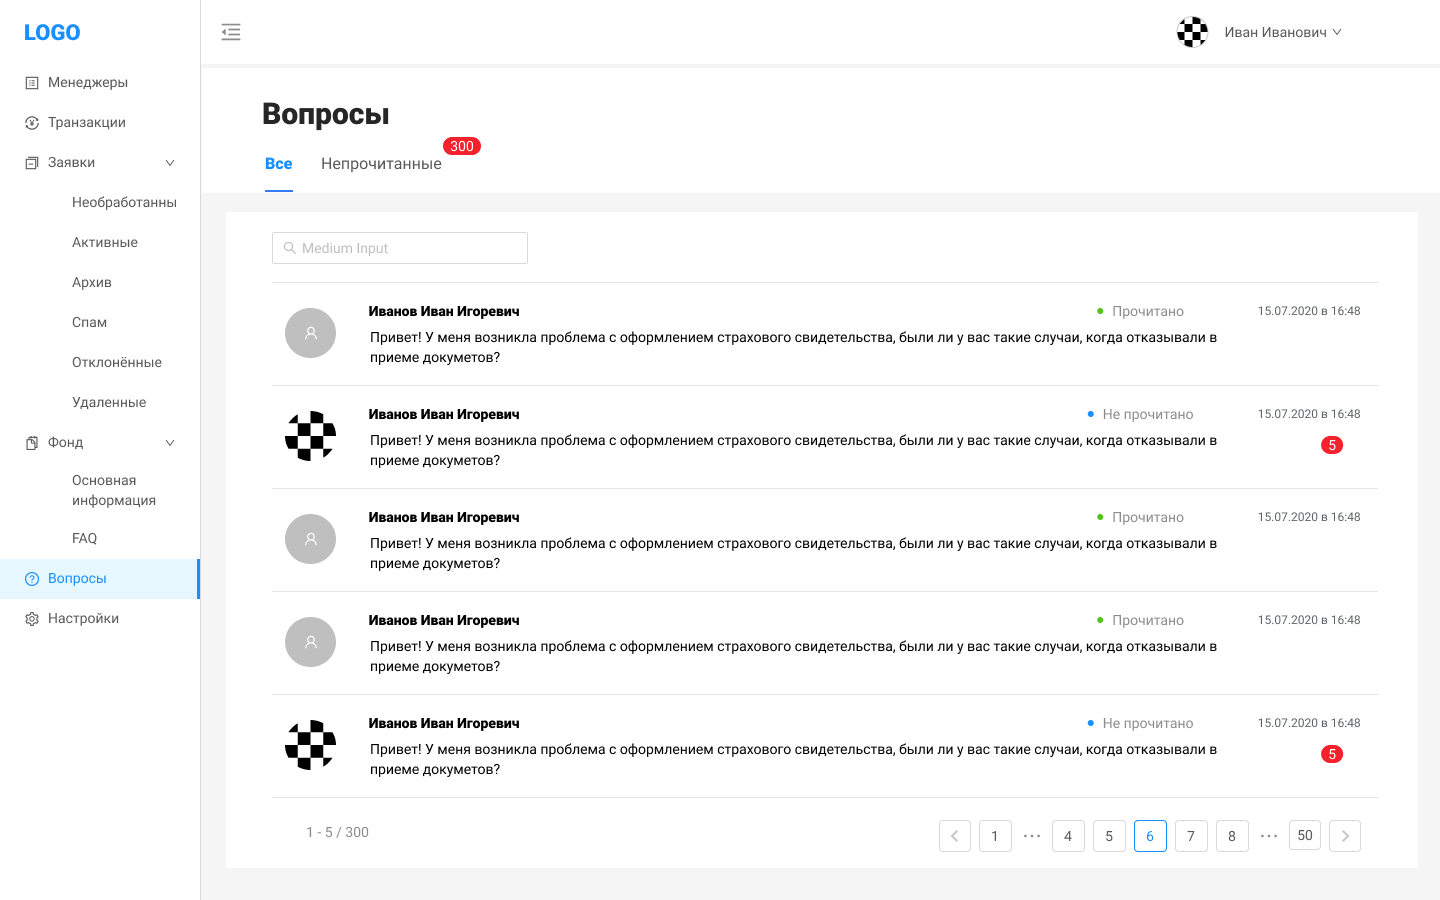
\includegraphics[width = 0.9\linewidth]{img/chats.png}
		\caption{Макет списка диалогов}
		\label{pic: applications}
\end{figure}

\begin{figure}[H]
		\centering
		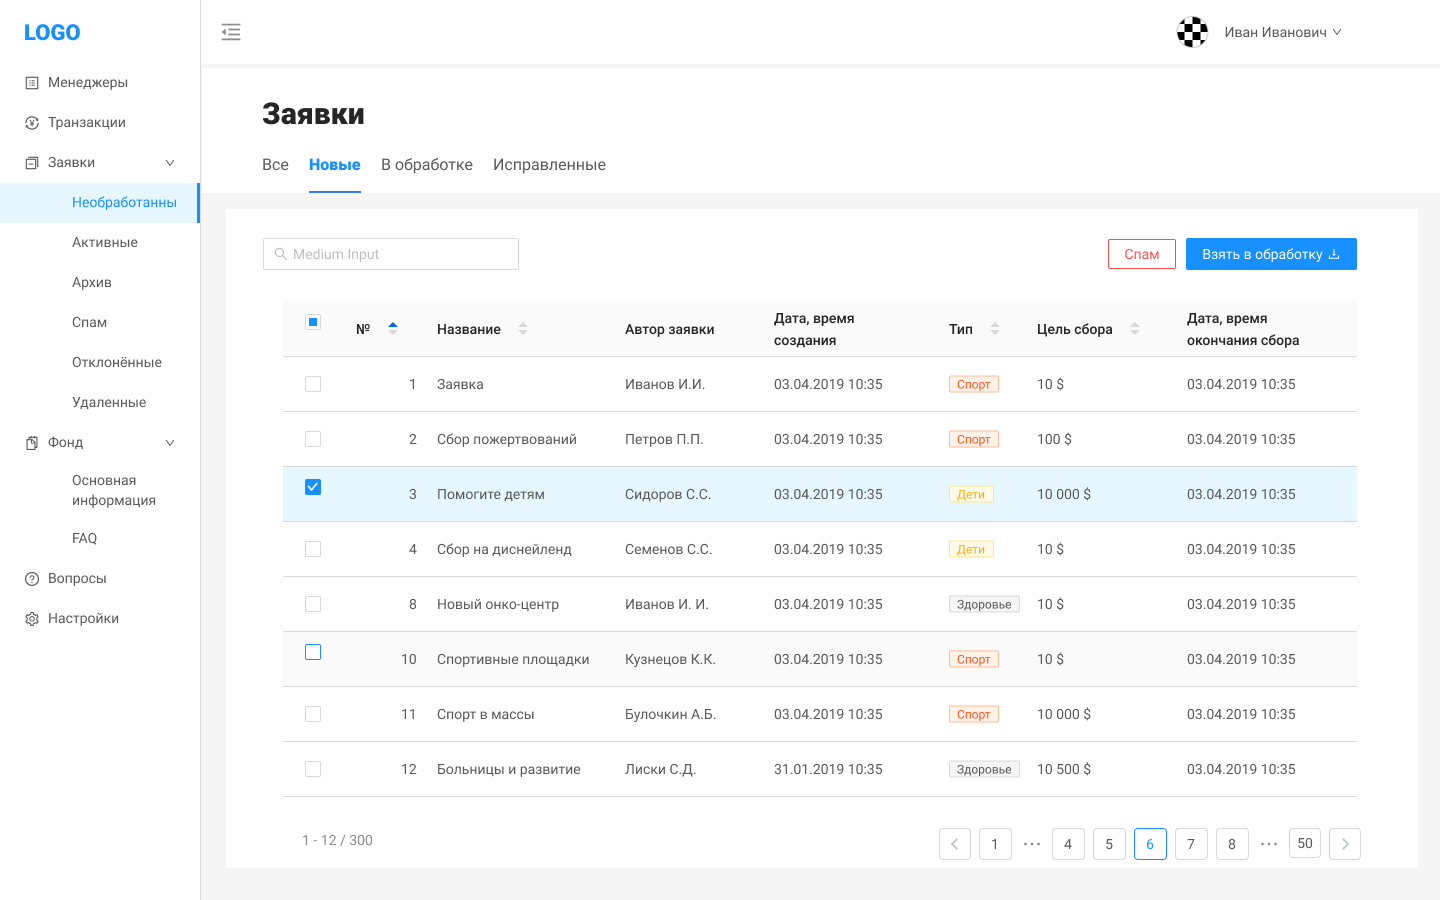
\includegraphics[width = 0.9\linewidth]{img/new.png}
		\caption{Макет списка заявок}
		\label{pic: applications}
\end{figure}

\begin{figure}[H]
		\centering
		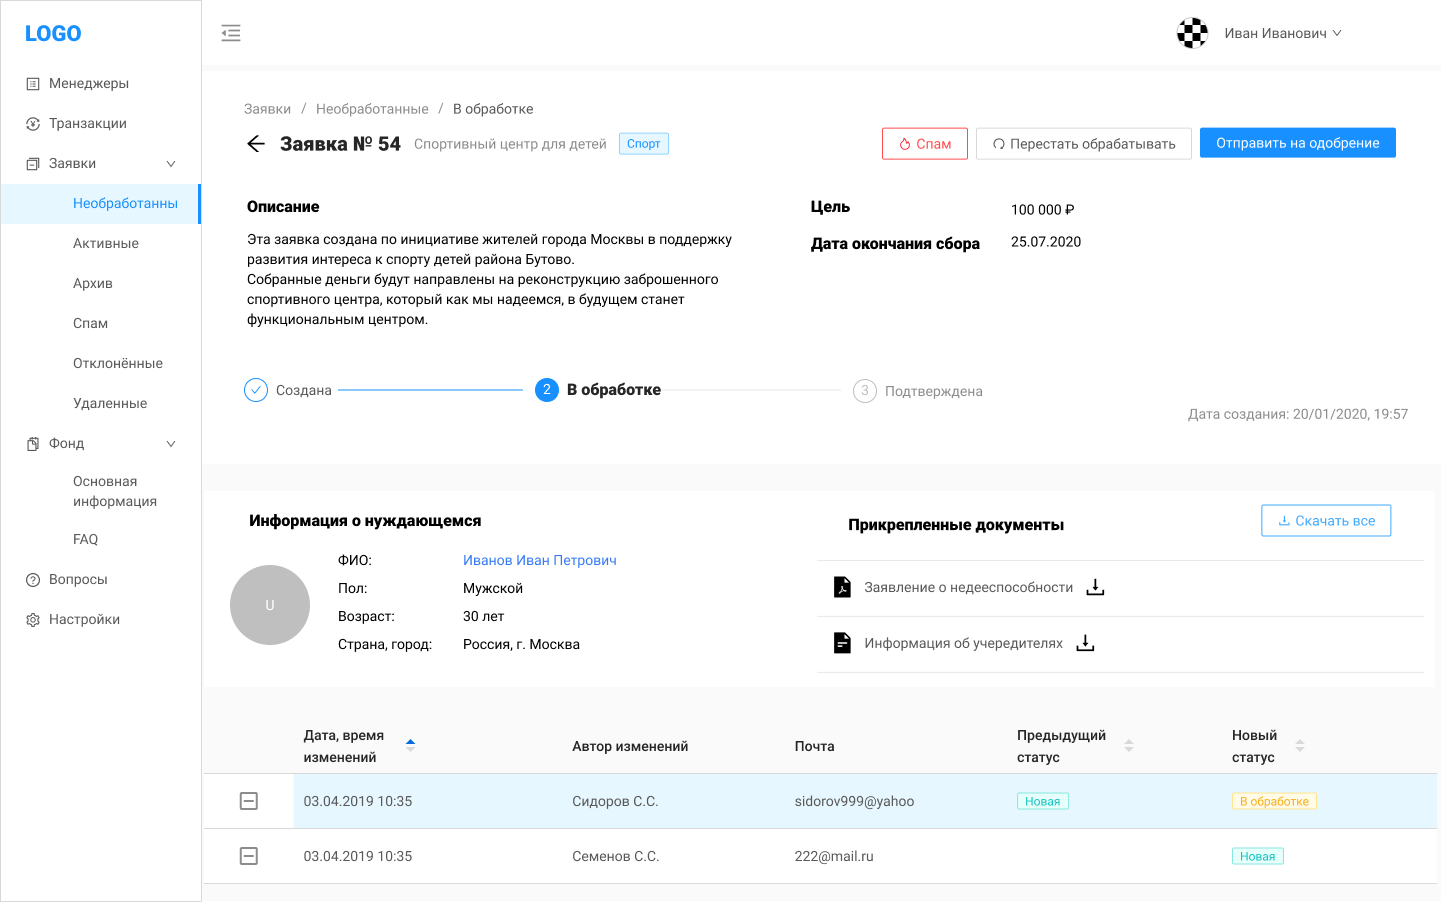
\includegraphics[width = 0.9\linewidth]{img/in-processing.png}
		\caption{Макет заявки}
		\label{pic: applications}
\end{figure}
	
	\newpage
	\addition{Ключевые прецеденты}{keyUsecase} 
	\begin{figure}[H]
		\centering
		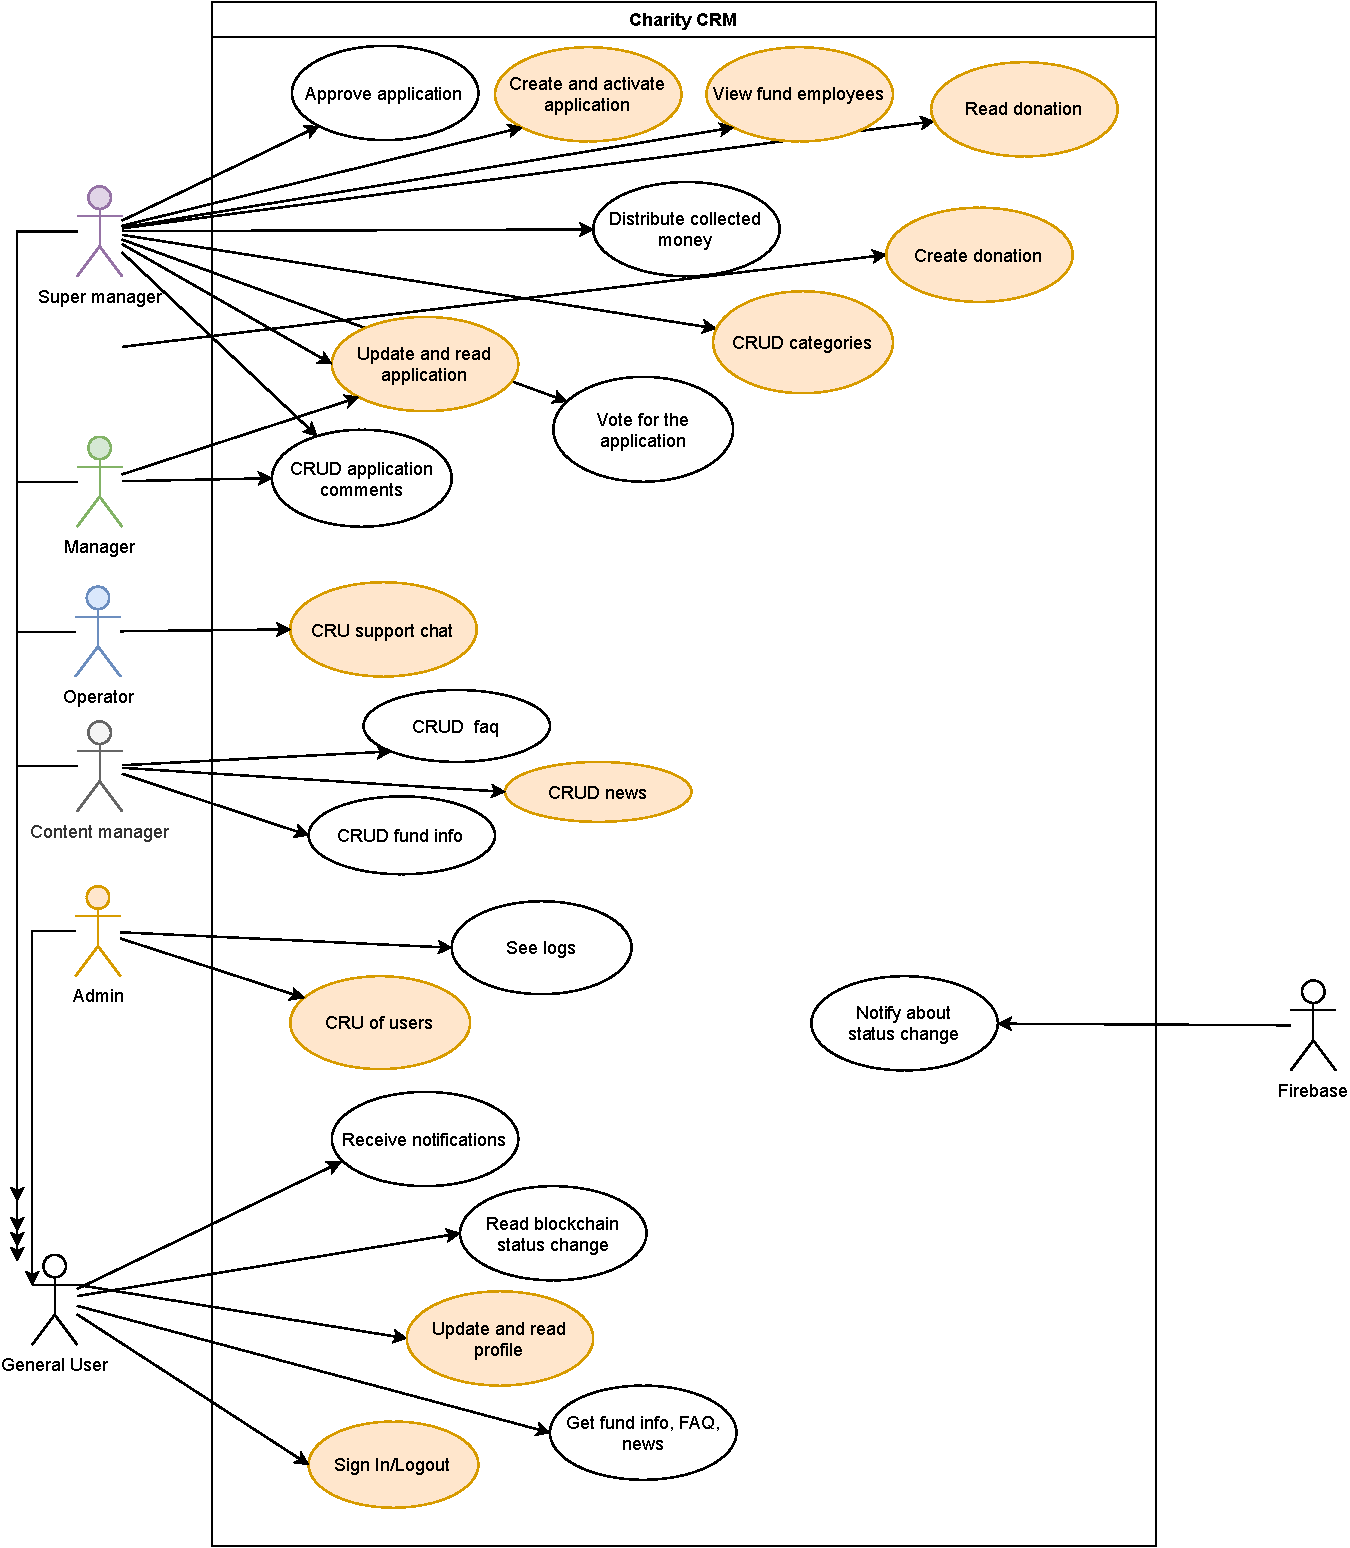
\includegraphics[width = 0.9\linewidth]{img/key-usecase.pdf}
		\caption{Диаграмма прецедентов}
    \end{figure}
    
    \newpage
	\addition{Тест кейс активации заявки}{test_1}
	
	\begin{figure}[H]
		\centering
		\begin{subfigure}[b]{0.475\linewidth}
			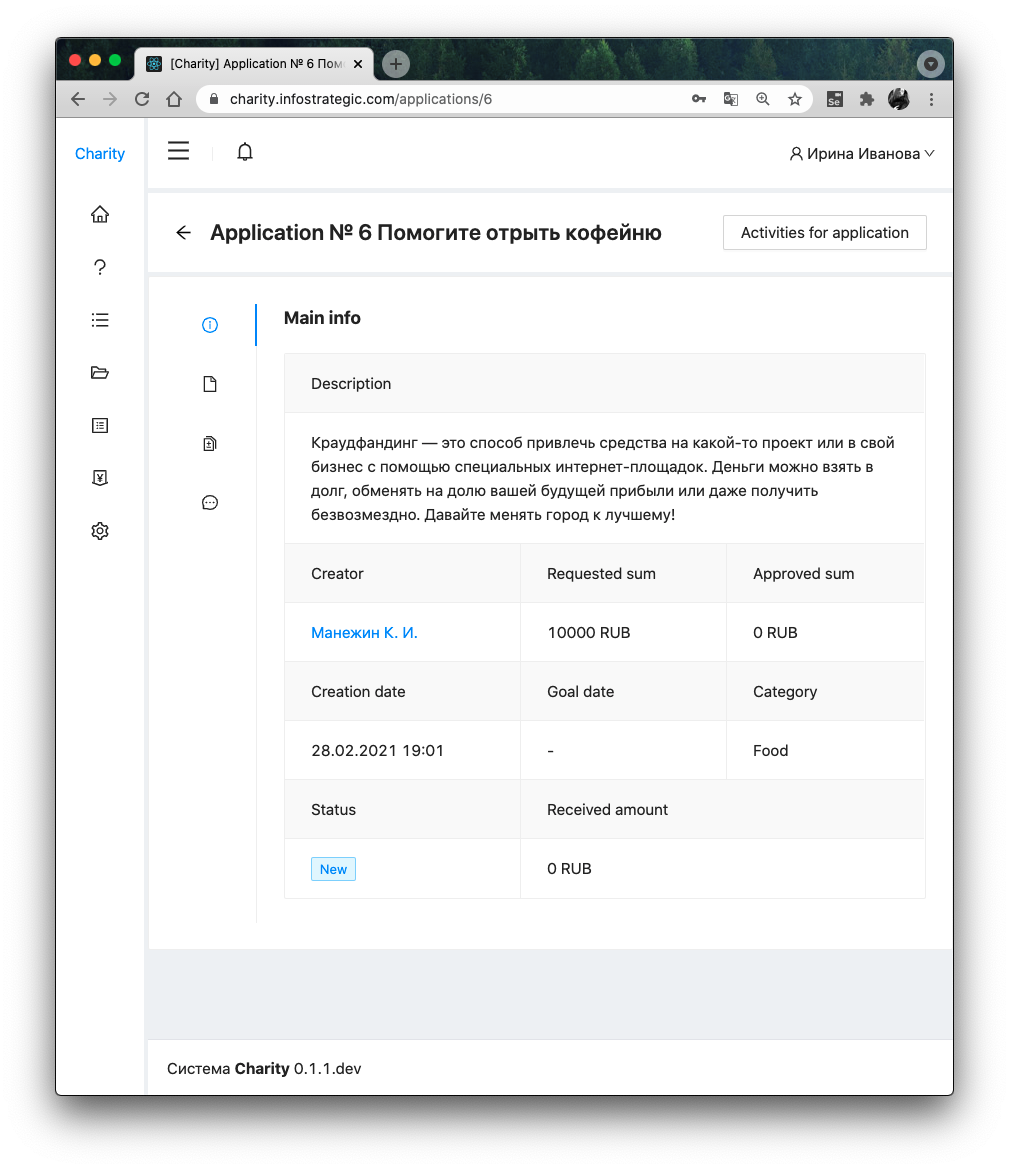
\includegraphics[width=\linewidth]{img/test/1.png}
		\end{subfigure}
		\begin{subfigure}[b]{0.475\linewidth}
			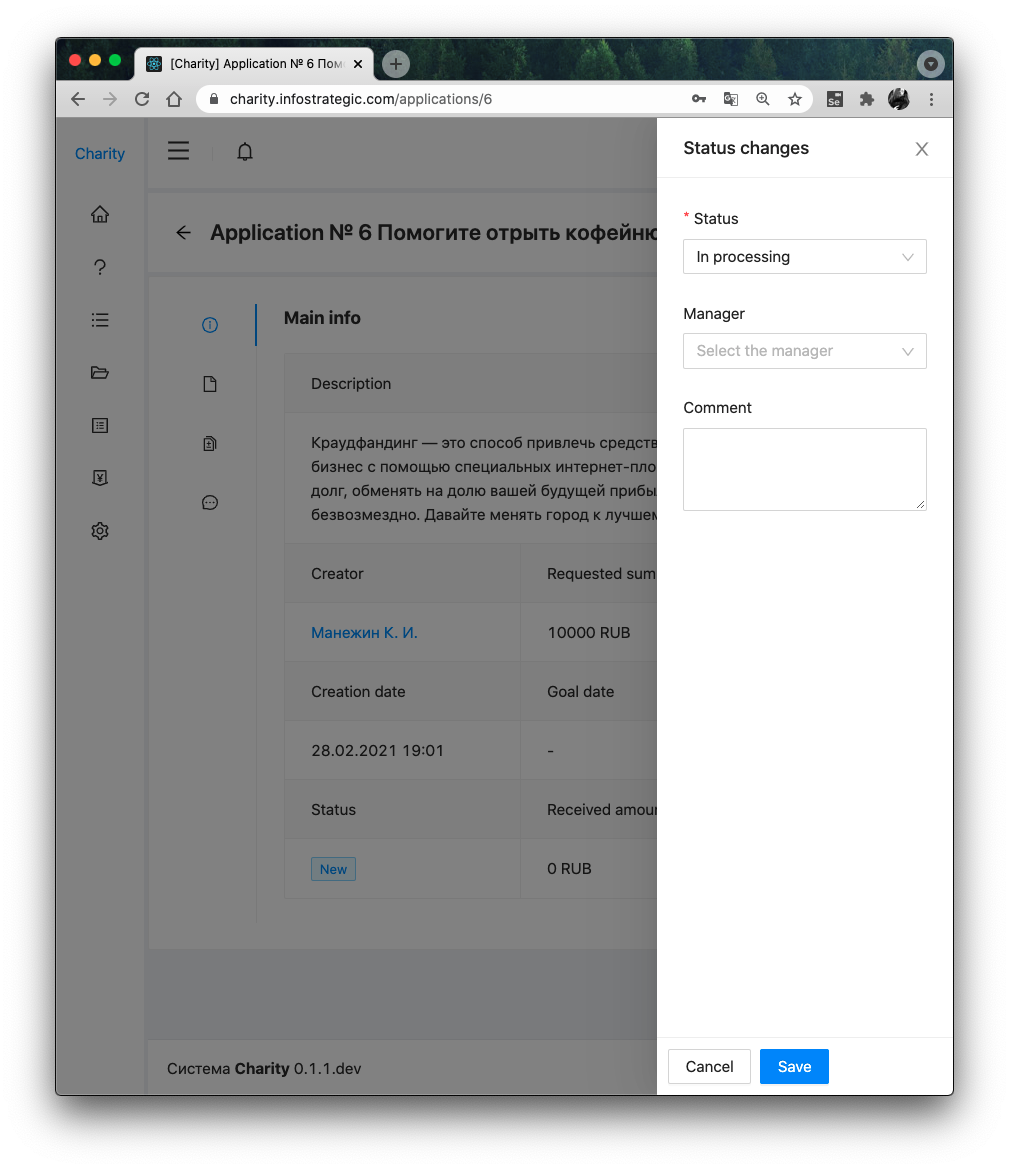
\includegraphics[width=\linewidth]{img/test/2.png}
		\end{subfigure}
		\begin{subfigure}[b]{0.475\linewidth}
			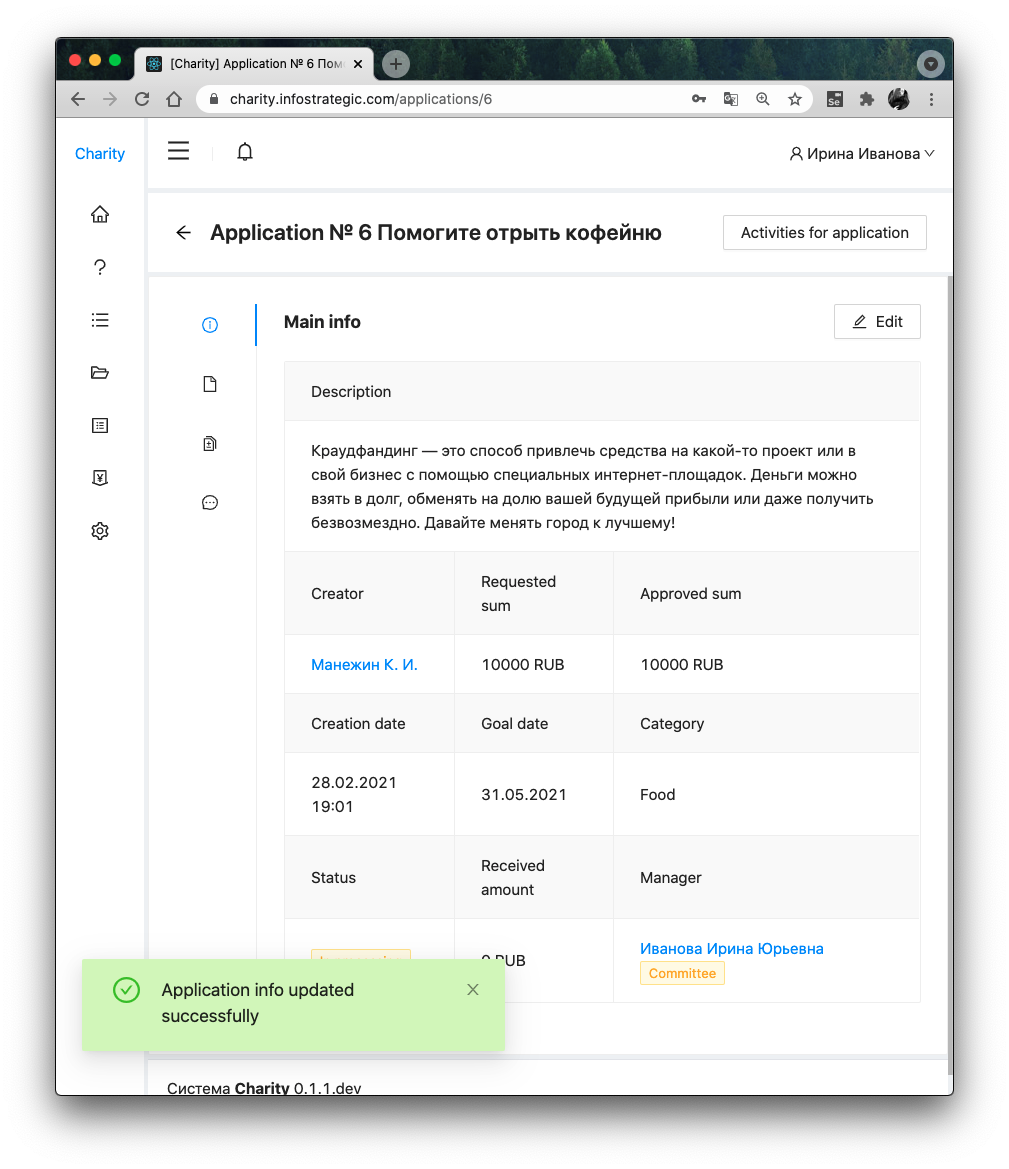
\includegraphics[width=\linewidth]{img/test/3.png}
		\end{subfigure}
		\begin{subfigure}[b]{0.475\linewidth}
			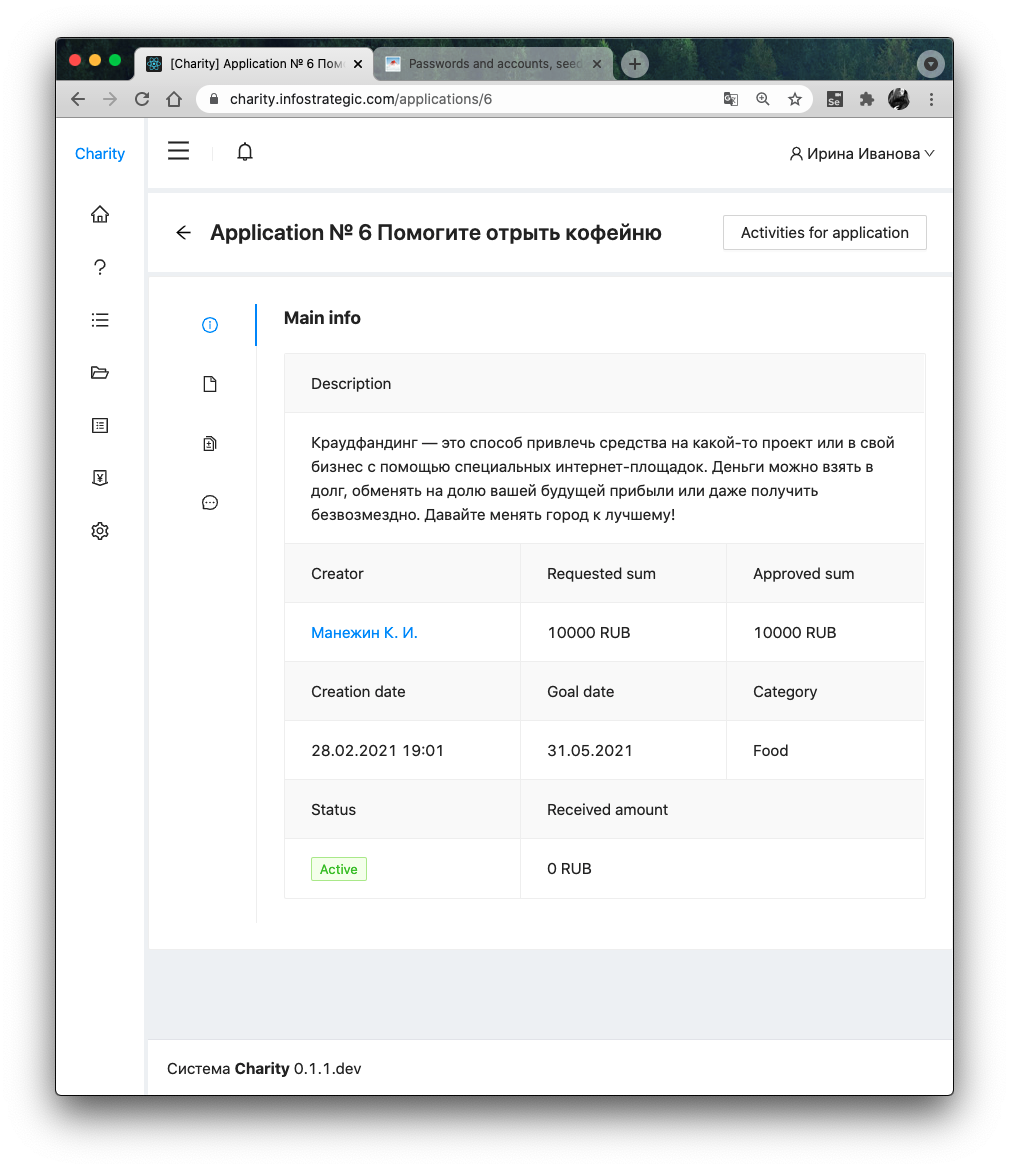
\includegraphics[width=\linewidth]{img/test/4.png}
		\end{subfigure}
		\caption{Скриншоты проведенного тестирорования TC-9}
	\end{figure}
	
		\newpage
	\addition{Тест кейс голосования по заявке}{test_2}
	
	\begin{figure}[H]
		\centering
		\begin{subfigure}[b]{0.475\linewidth}
			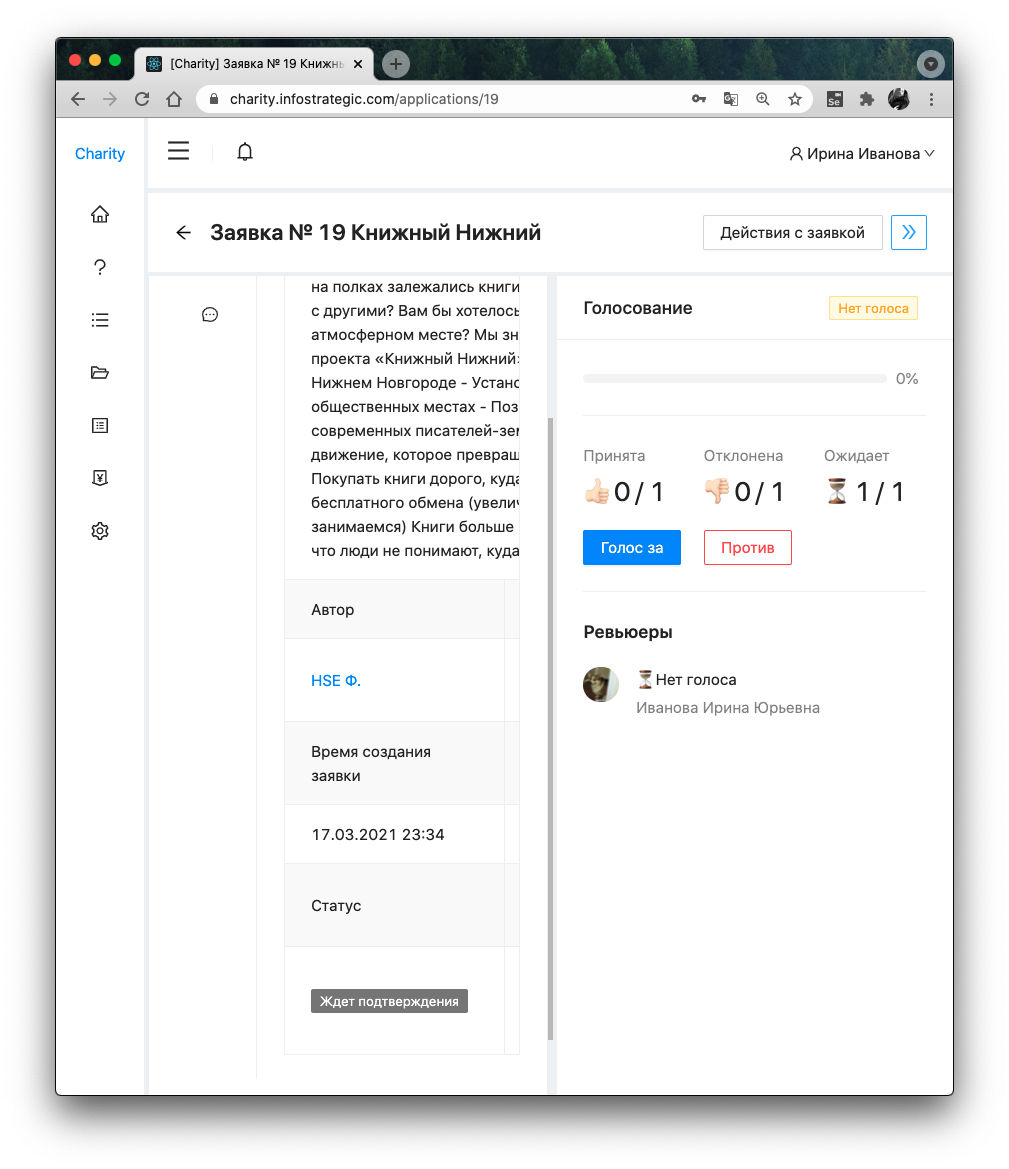
\includegraphics[width=\linewidth]{img/test/5.png}
		\end{subfigure}
		\begin{subfigure}[b]{0.475\linewidth}
			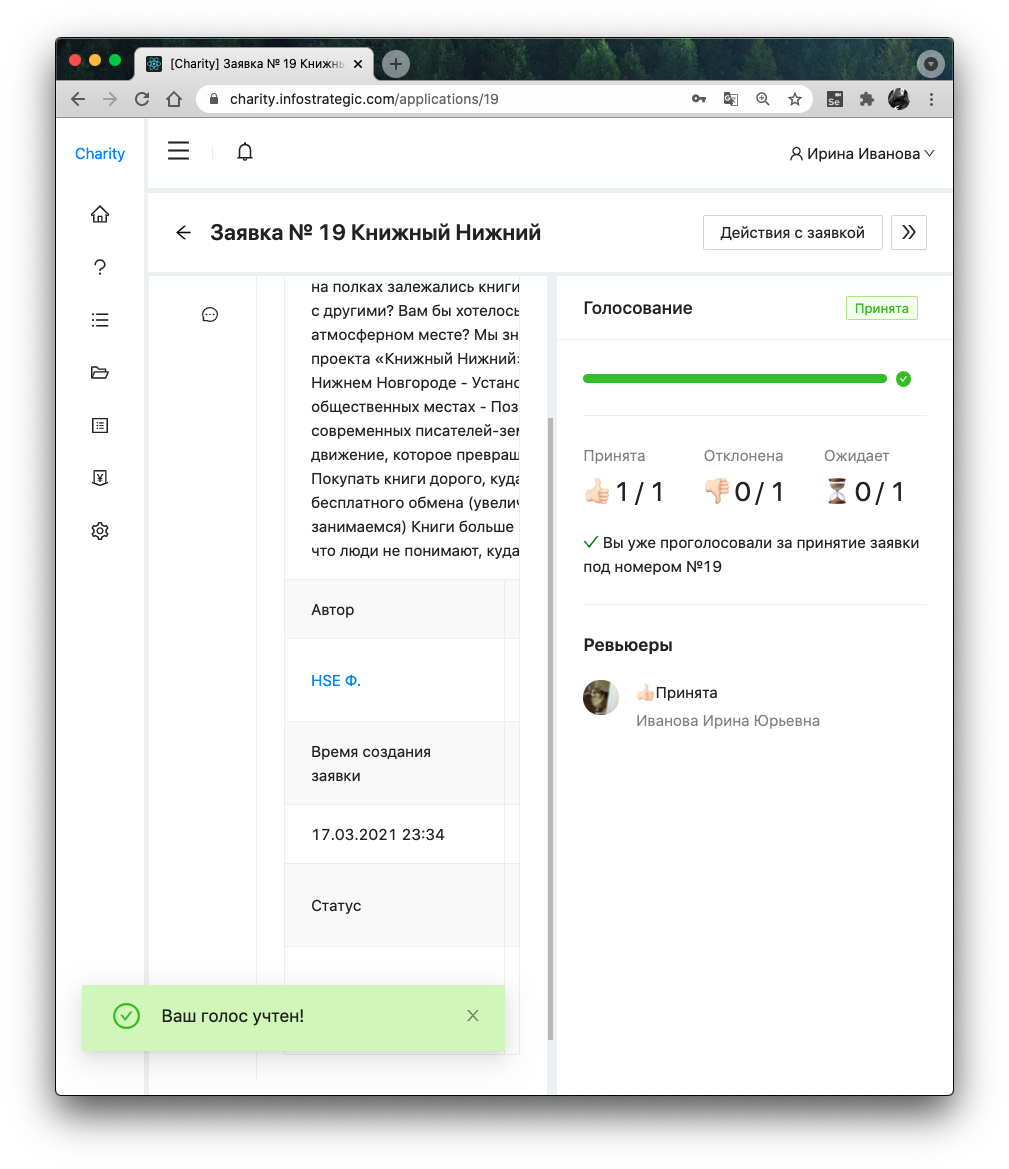
\includegraphics[width=\linewidth]{img/test/6.png}
		\end{subfigure}
		\begin{subfigure}[b]{0.475\linewidth}
			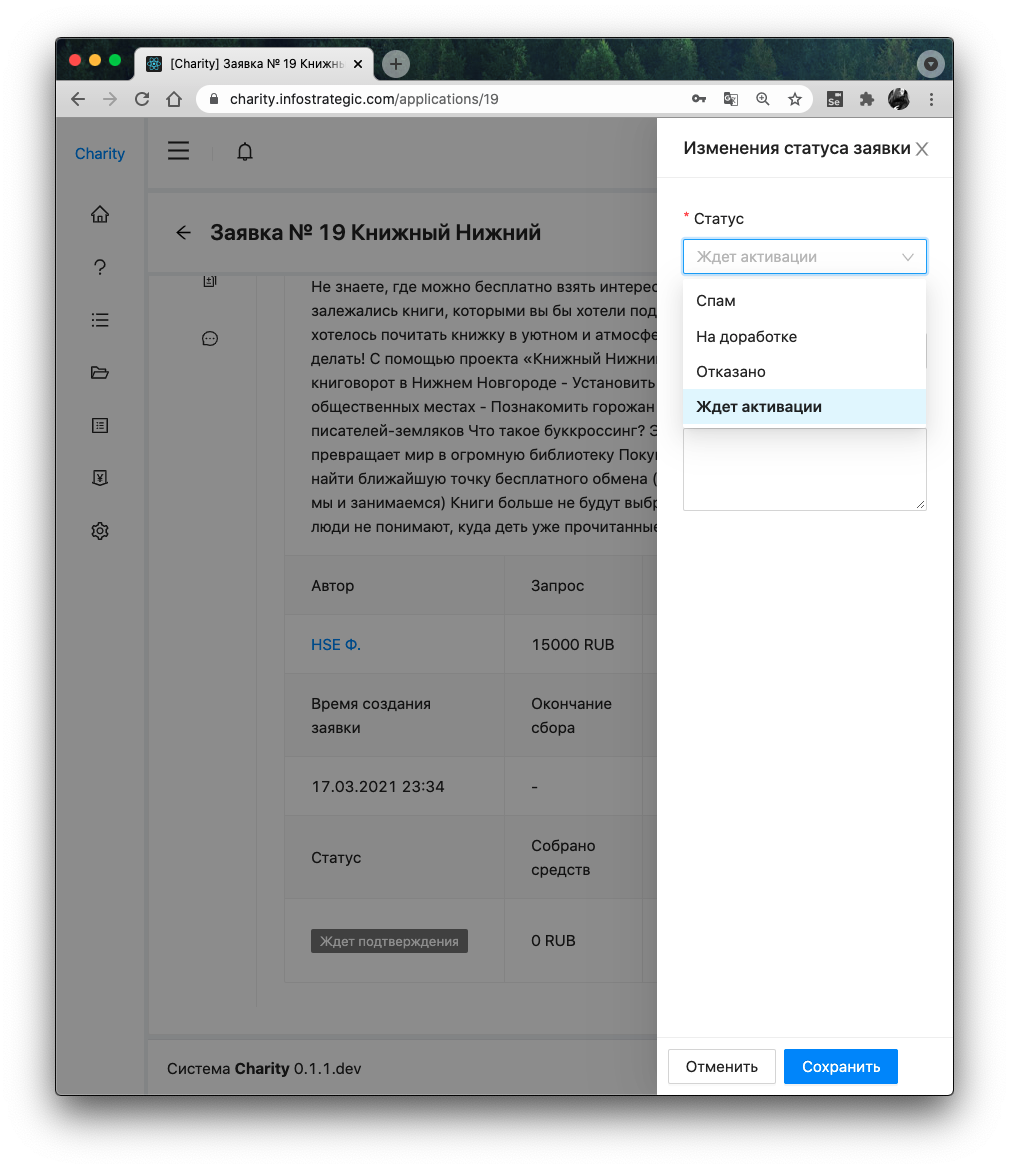
\includegraphics[width=\linewidth]{img/test/7.png}
		\end{subfigure}
		\caption{Скриншоты проведенного тестирорования TC-10}
	\end{figure}
	
	\newpage
	\addition{Роли сотрудников фонда}{stuff}
	\begin{description}
		\item[\textbf{Администратор}] -- это сотрудник фонда, который имеет доступ к функционалу по управлению пользователями системы.
		\item[\textbf{Член комиссии}] -- у каждого фонда есть комиссия, которая принимает итоговое решение об активации заявок от нуждающихся. В обязанности членов комиссии также входит обработка заявок, просмотр пожертвований поступающих от доноров, создание категорий для заявок и так далее.
		\item[\textbf{Контент-менеджер}] -- отвечает за управление контентом фонда, а именно: часто задаваемыми вопросами, основной информацией фонда и новостями фонда;
		\item[\textbf{Менеджер}] -- большая часть сотрудников фонда состоит из менеджеров фонда. В их обязанности входит только обработка заявок, коммуникация с пользователями и сбор необходимых документов если требуется;
		\item[\textbf{Оператор}] -- оператор фонда отвечает на вопросы пользователей мобильного приложения;
\end{description}
	
	\newpage
	\addition{Диаграмма жизненного цикла заявки}{status} 
	
	\begin{figure}[H]
		\centering
		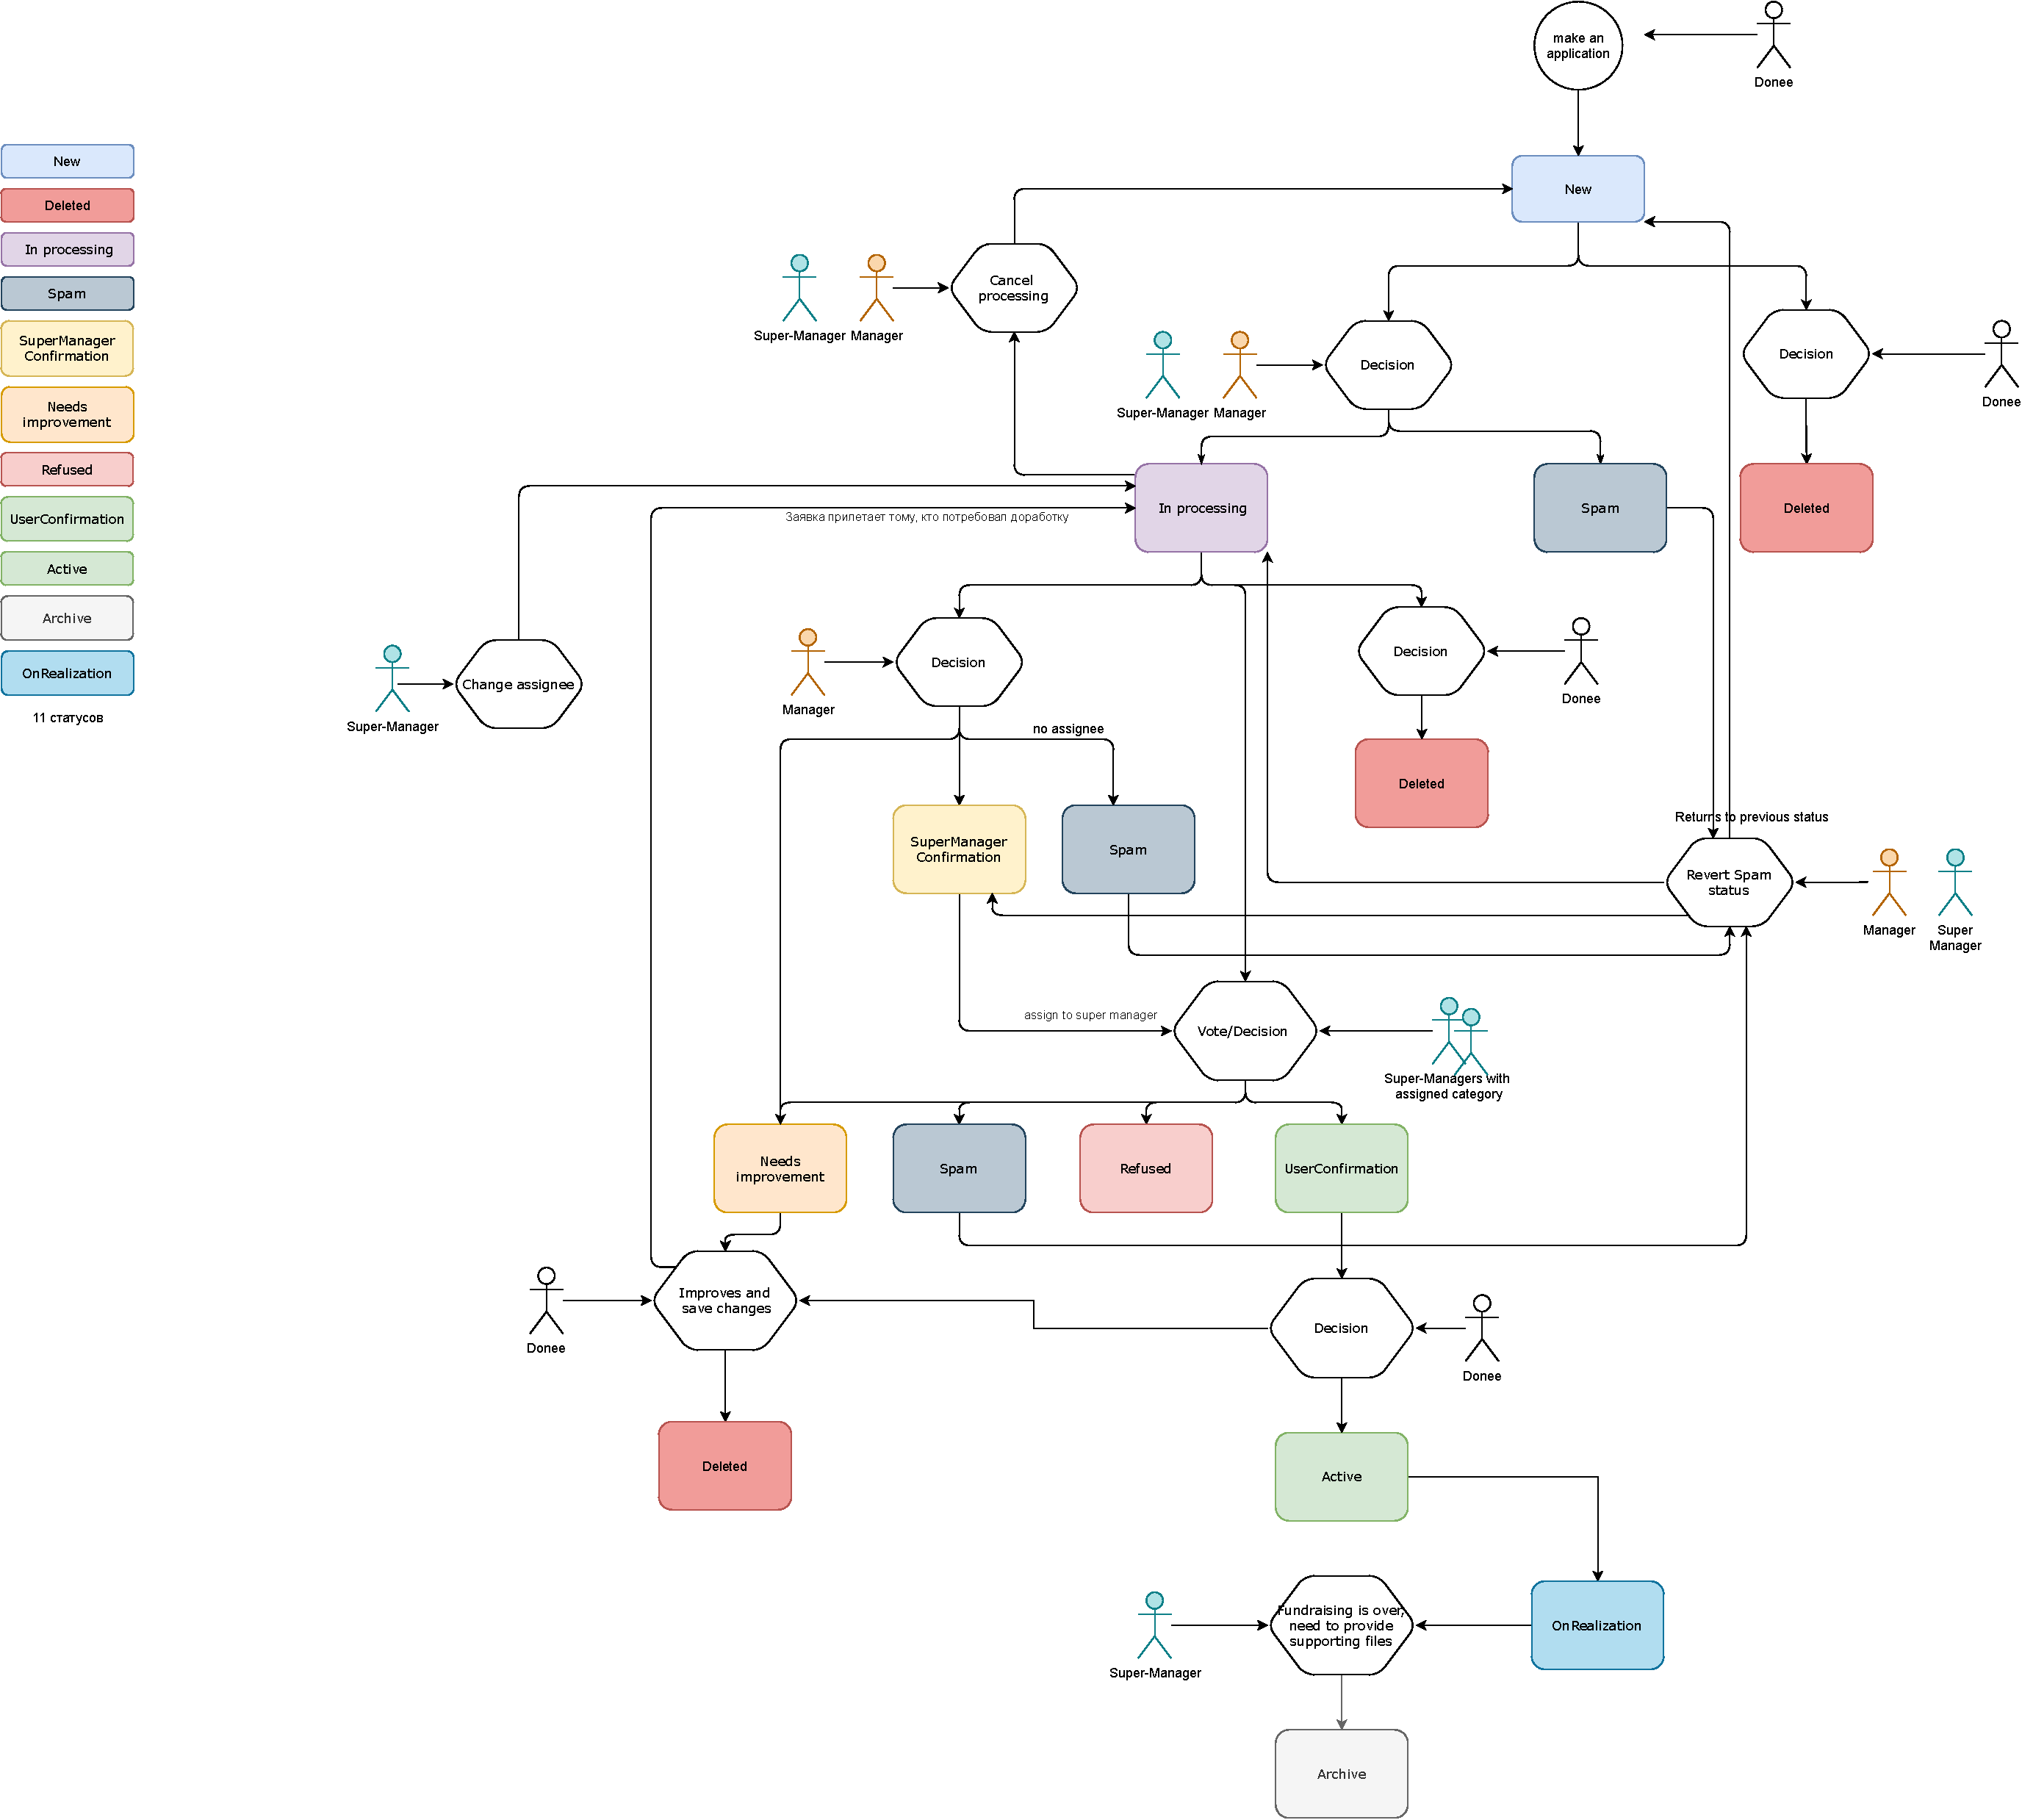
\includegraphics[width = 0.9\linewidth]{img/statusflow.pdf}
		\caption{Диаграмма статусов}
		\label{pic: status}
	\end{figure}
	
	
	
	\newpage
	\listRegistration
	
\end{document}